\chapter{Object-Oriented Analysis \& Design} \label{chapter:chapter4}

Object-Oriented Analysis (OOA) is a key activity in good software design as it facilitates the difficult transition between the problem domain and the solution domain. During this stage in the development process, the designer switches from a user-centric to an object-oriented point of view. Information from the domain model, use cases and requirements is extracted and systematically translated into a conceptual model. While the analysis is concerned with the "what", the design focuses on the "how" of a system.

The design phase refines the analysis model and describes the objects, their attributes, behaviour, and interactions in detail. Outputs of the design model should, therefore, include all details necessary to implement the product. However, Object-Oriented Analysis and Design activities are best conducted in iterative and incremental steps. 

In the following section we will elaborate on the analysis model and on how this output shapes the subsequent design model.

% ==============================================================================
%                              ANALYSIS DIAGRAM SECTION 
% ==============================================================================
\section{Analysis Model}

The goal of the analysis model is to create a draft version of the system. Although it abstracts the definition of the most important objects, the analysis model should exhaustively capture the system's required entities. Therefore, a data-driven design approach to identifying all classes was taken.

\begin{figure}[H]
    \centering
    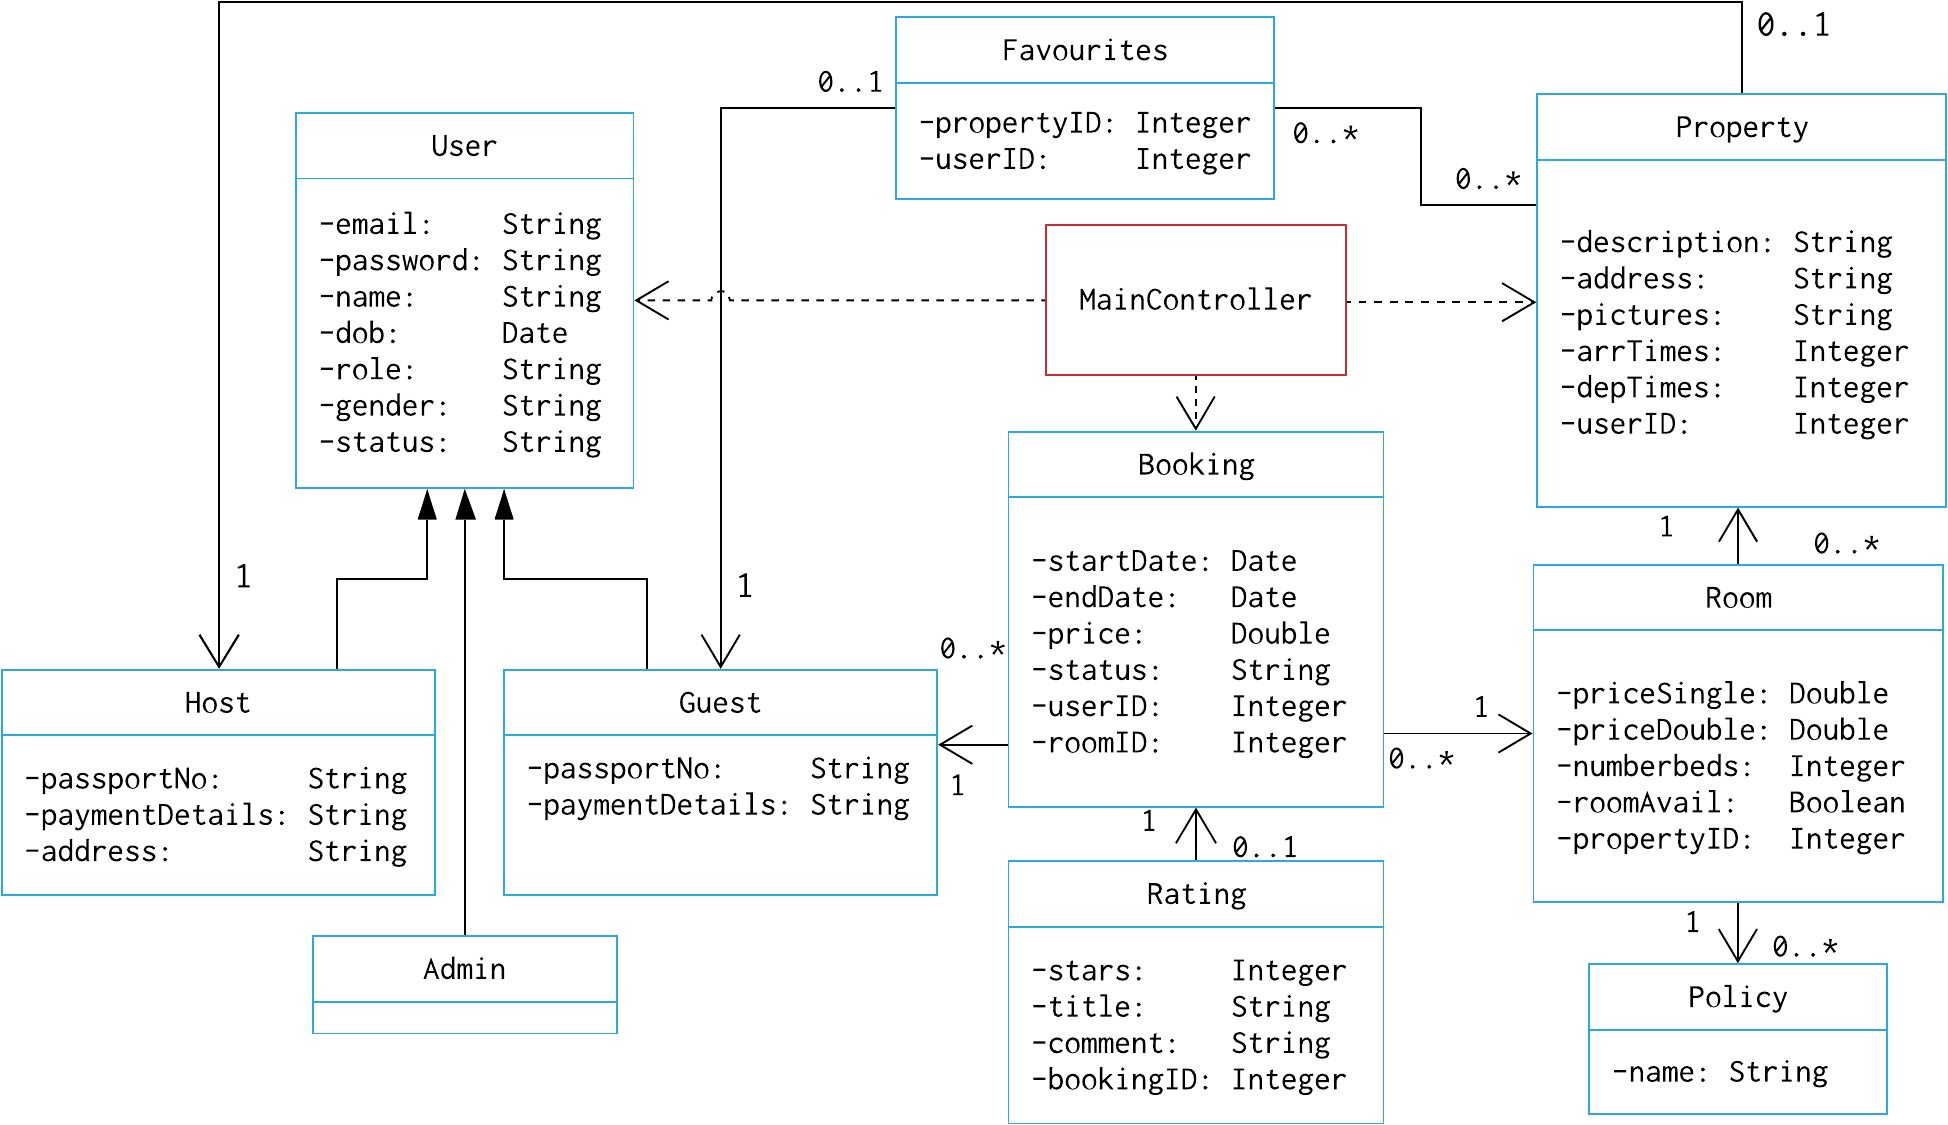
\includegraphics[height=9.5cm]{img/analysis_diagram.png}
    \caption{Analysis Class Diagram}
    \label{analysis_diagram}
\end{figure}

After locking down the requirements and subsequently the use cases, the entity classes in the system were identified, as shown in figure \ref{analysis_diagram}. This was achieved by extracting the main nouns that were being commonly used, such as: \texttt{User}, \texttt{Property}, and \texttt{Booking} \cite{GangOfFour1994}.

The Analysis Class Diagram displays the initial classes in the B\&B system and indicates the multiplicities and associations between them. The model achieves high cohesion by acknowledging the separation of concerns design principle, therefore assigning only a small and well-defined set of responsibilities to each class.

% ==============================================================================
%                              DESIGN DIAGRAM SECTION 
% ==============================================================================
\section{Design Model}
The Design Class diagram shown in figure \ref{design_diagram}, illustrates a more interconnected architecture than that shown in figure \ref{analysis_diagram}. This diagram's main purpose is to show the classes and their relationships, in addition to their attributes and operations. The system's architecture is made up of a mix of the following types of UML classes: Boundary, Entity, Controller, and Enumeration. It is to be noted that many of the parameters are abbreviated terms from our glossary for brevity.

As shown by the legend in figure \ref{design_diagram}, the classes have been colour-coded according to the class group that they belong to. The system has been designed to comply with the \textbf{Model-View-Controller} pattern, which will be discussed in more detail in section \ref{component_section}.

\begin{itemize}
    \item \textcolor{RoyalBlue}{\textbf{Models/Entity Classes}}: These classes have a connection to the database. By using Object-relational mapping, their objects can be modelled as database records that include attributes and operations that are mainly CRUD based \cite{Hibernate}. Any additional business logic will also be placed in these classes.
    Getter and setter operations such as \texttt{User.getName()}, which returns the name attribute of a given user object, have been left out of the diagram due to space constraints. They are implicitly included in the rest of the sequence diagrams in section \ref{sequence_section}.

    \item \textcolor{red}{\textbf{Controller/Control Classes}}: These classes provide endpoints to the users in the form of actions. Every HTTP request made by the browser will be connected to an appropriate operation under these classes.
    \item \textcolor{RedViolet}{\textbf{View Classes}}: After various meetings with the client, the recommendation that was decided on was to add these types of classes which are responsible for generating the HTML to be displayed by the browser. They receive parameters from the appropriate controllers in the form of objects.
    \item \textcolor{LimeGreen}{\textbf{Boundary Classes}}: Within the system, there exists a need to talk to external services such as email service providers and payment gateways. The boundary classes act as the connection between these services and the internal models and controller. The connection is achieved by sending requests and receiving success/failure responses.
    \item \textcolor{Goldenrod}{\textbf{Enumeration Classes}}: These classes represent a common type of data as constants.
\end{itemize}

\begin{figure}[H]
    \centering
    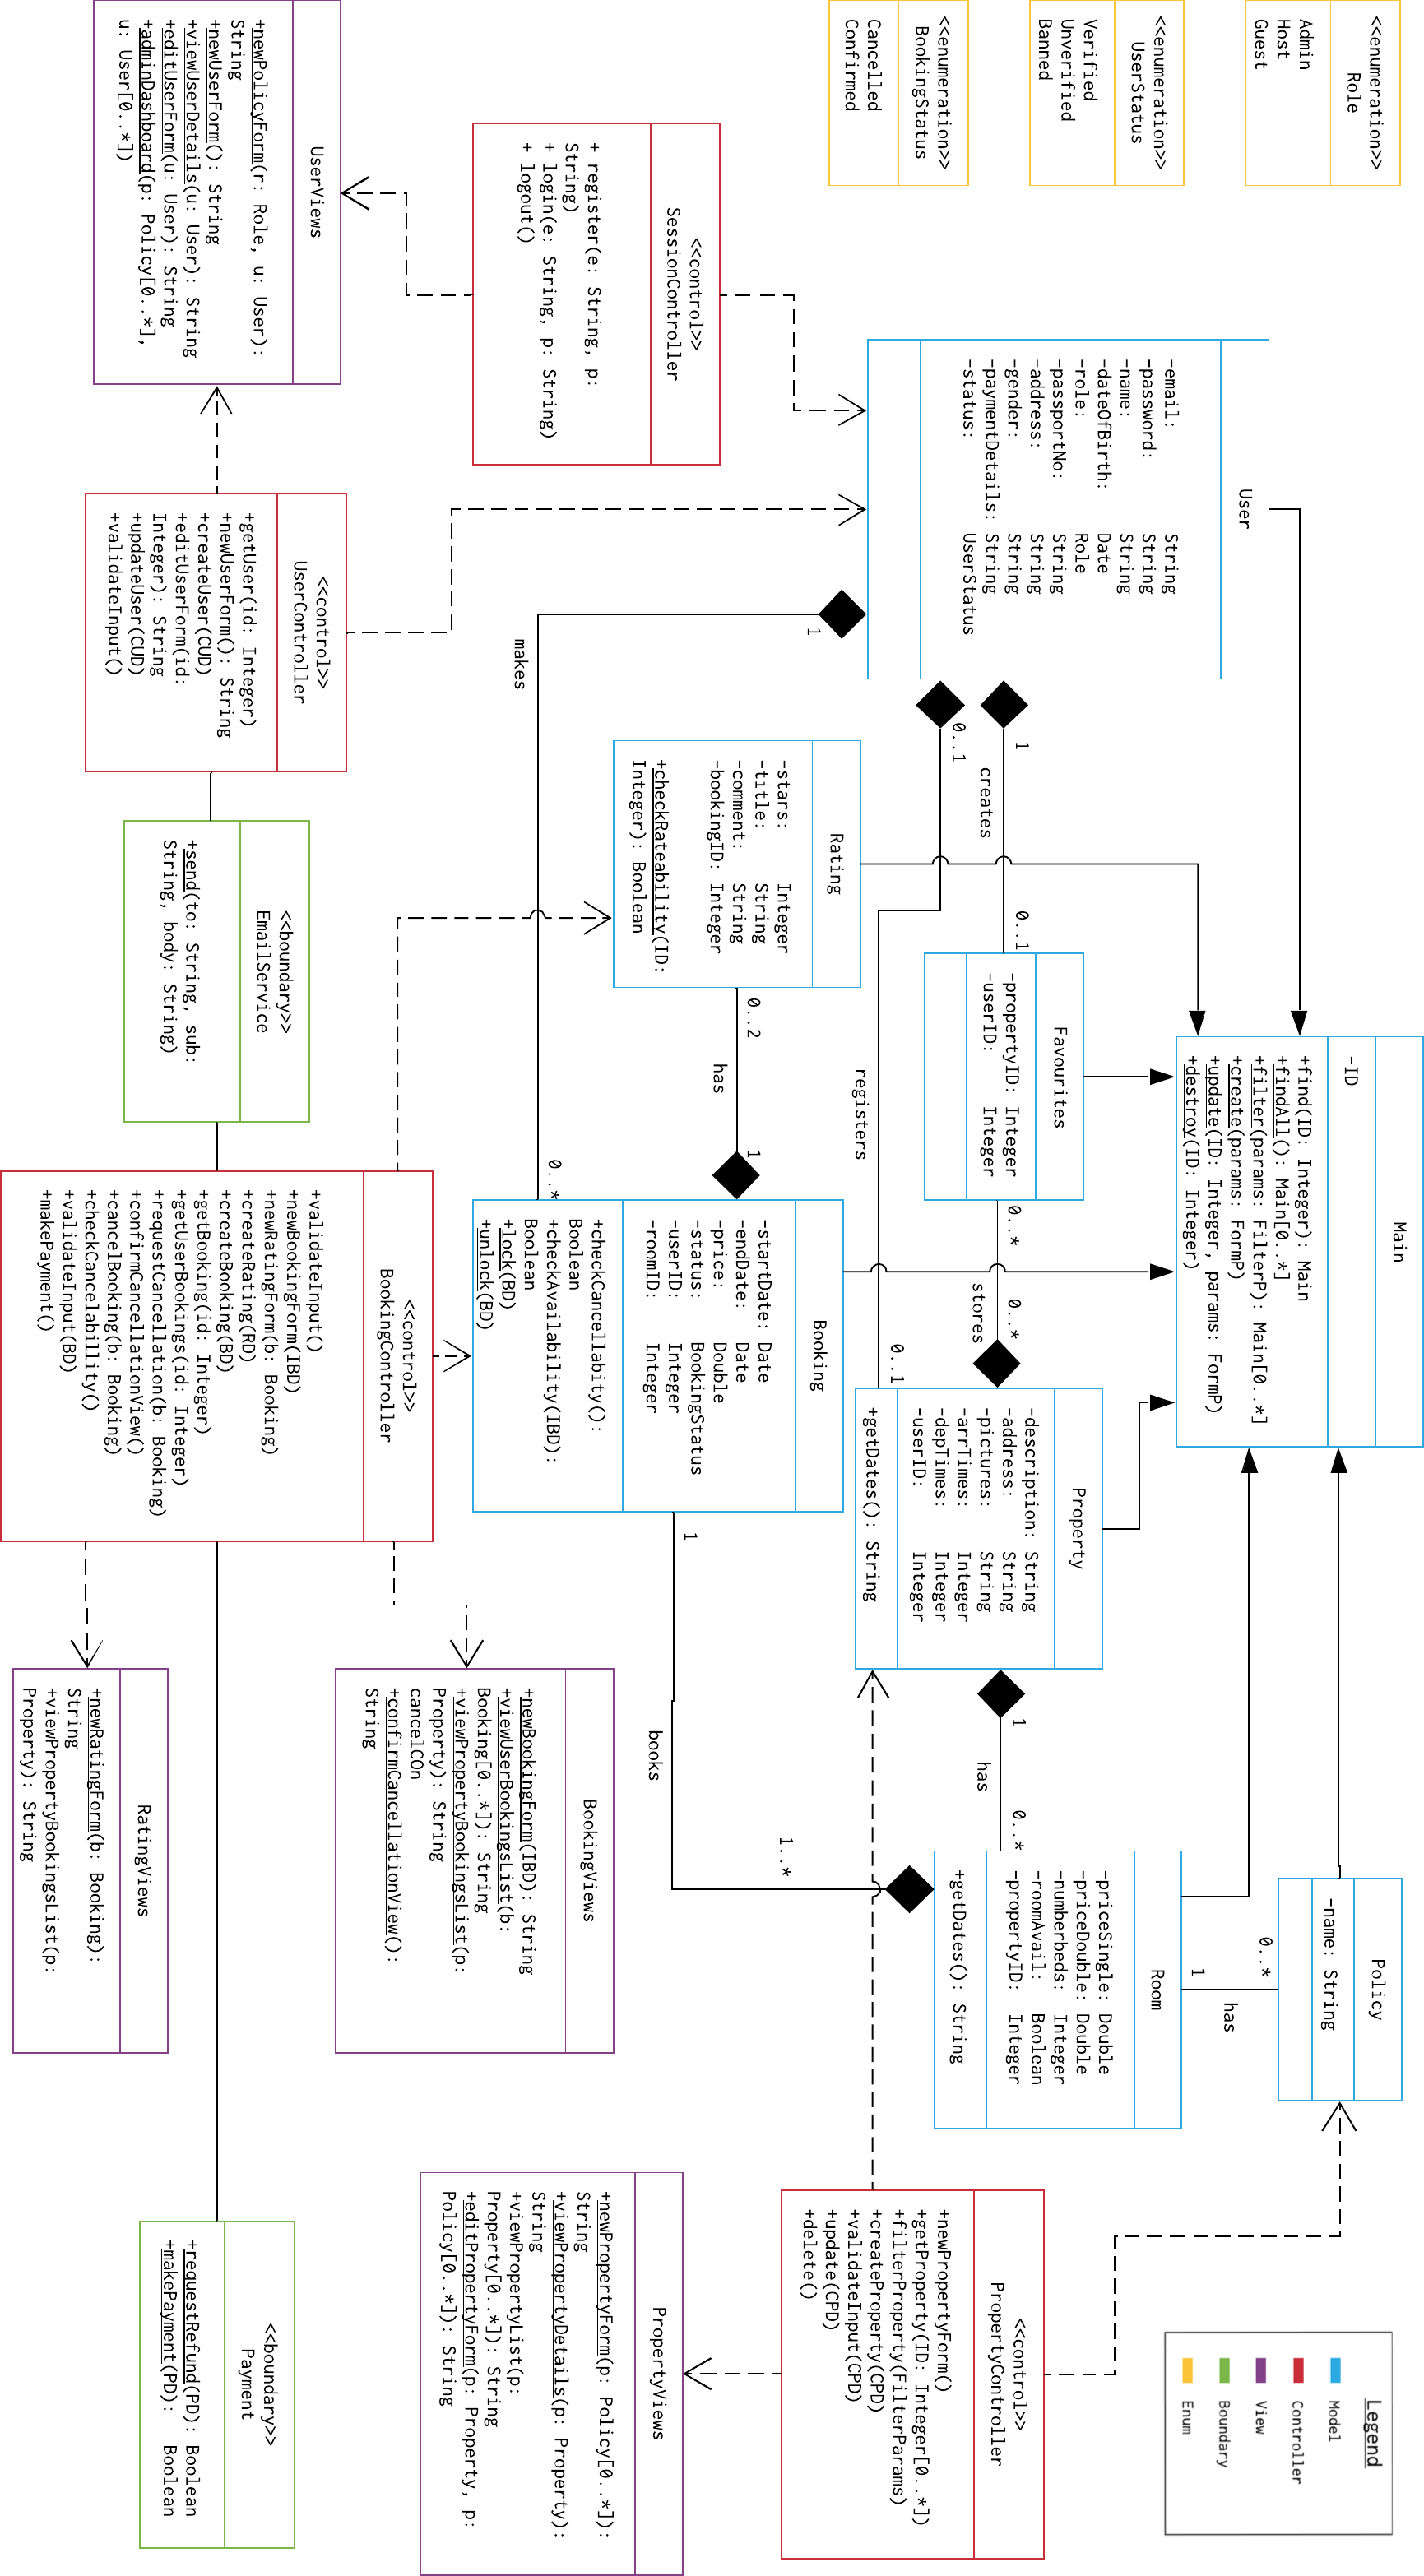
\includegraphics[width=14cm]{img/design_diagram_h.png}
    \caption{UML Design Class Diagram}
    \label{design_diagram}
\end{figure}

% ==============================================================================
%                              SEQUENCE DIAGRAM SECTION 
% ==============================================================================
\section{Sequence Diagrams} \label{sequence_section}

Sequence diagrams are valuable tools for specifying how use cases can be implemented by the system in line with the classes, controllers, views, and methods developed in the class diagram. Specifically, they show the explicit sequence in which messages between the interacting parties in a use case are exchanged. The six sequence diagrams presented in this work do not fully exhaust all possible options of a given use case which would constitute a generic form, but rather depict some specific scenario or route through the use case \cite{George2017}.\footnote{Most scenarios chosen were straightforward success routes, but note that Figure \ref{Sequence Diagram: View Property List} (View Property List) portrays two iterations of a Property search loop, with one iteration coming up with an empty result set and hence showing the User a warning notification.}

Following the agile approach, the sequence diagrams have been developed iteratively with the intention of striking a balance between the level of detail for implementation in code and degree of abstraction to emphasize the core concepts (see the more detailed notes on this below).

All the methods and classes listed in the sequence diagrams correspond to the information in the class diagram. Return values that are pure HTML strings, e.g. the details of a property, are denoted as views, i.e. \texttt{propertyDetailsView}.

Note the following about the presentation here:

\begin{itemize}
    \item The class name has been used when referring to the class itself (this usually happens when using the class' static methods), and an object name followed by a colon and a class name when referring to an object (so, for instance \texttt{Property} is the Property class, whereas \texttt{p : Property} is a Property object.)
    \item When sending a message to some external actor or system (such as the Payment System in Table \ref{Sequence Diagram: Make Booking} (Make Booking)), the text associated with the message is not meant to name a method --- it is simply a description of the message.
    \item The parameters of the method calls are not in any strict format --- it should be clear from the context what is being sent at each stage. Abbreviations of terms from the glossary are commonly referred to as done in the Design Class Diagram. Note also that some of the methods are overloaded (it should always be clear from the context how this works --- \texttt{validateInput()} method in \texttt{BookingController} can check both Booking Details and Initial Booking Details in the obvious way)
    \item Each diagram includes a list of the use case Main Flow steps (for example, "P-C.3.a.") corresponding to each of its stages at the very left. Duration lines (the lines with dots at either end) are also attached to the steps to make things even clearer.
    \item The diagrams have been simplified: due to space and legibility constraints, we have left out many lower-level method calls necessary to carry out the represented scenarios. A typical example of this is the Property constructor call in Figure \ref{Sequence Diagram: Register Property} (Register Property). In a more detailed depiction, the constructor would loop over all the Rooms in the Property constructing each of them, and then further loop over all Policies in each of the Rooms, constructing each of those as well. The current diagram is much clearer than one involving nested loops would be, and the intended realization in terms of lower-level method calls is obvious. Another example of simplification: the static database-related method calls made to the Model classes (\texttt{filter()}, for instance) are shown as returning objects of the same classes. The group thought it clear that a constructor was being called in such instances, and thought it would be unnecessary to add such details to the diagrams.
    \item In a similar vein, it is sometimes implicitly assumed that certain pieces of information can be accessed (in cases where it should be clear where this information comes from). This can be illustrated with the User object \texttt{u} in Figure \ref{Sequence Diagram: Cancel Booking} (Cancel Booking) and the Payment Details in Figure \ref{Sequence Diagram: Make Booking} (Make Booking). In the former, it is assumed that \texttt{u} is already constructed, and it is used to get a set of Payment Details. The object corresponds to \texttt{aGuest}, the main actor in the diagram, and was obtained when \texttt{aGuest} logged in. Its reference is being held by a \texttt{SessionController} object. In Figure \ref{Sequence Diagram: Make Booking}, even the method call to the User object is skipped, and it's assumed that the Payment Details are already available. Assumptions like these helped make the diagrams much cleaner. (Another similar assumption in the same diagrams: the Users' email addresses are retrieved without explicitly fetching them at any point.)
    \item Many of the objects used are portrayed as being destroyed when the method that held their reference finishes executing (and hence there are no explicit destroy messages sent). In practice, when the objects are destroyed would depend on the garbage collection implementation of the finished application, but such details are not considered here.
    \item Note that in effect all the steps necessary to view a User's Bookings (see B-L-1 (Table \ref{use_case_B-L-1}) for the use case) are repeated in Figures \ref{Sequence Diagram: Make Booking}, \ref{Sequence Diagram: Cancel Booking} and \ref{Sequence Diagram: Give Rating}. This is due to all the portrayed scenarios finishing with a list of User Bookings. Use case inclusion would have made these diagrams simpler at the cost of potentially making our use cases more difficult to understand. 
\end{itemize}

\begin{figure}[H]
    \centering
    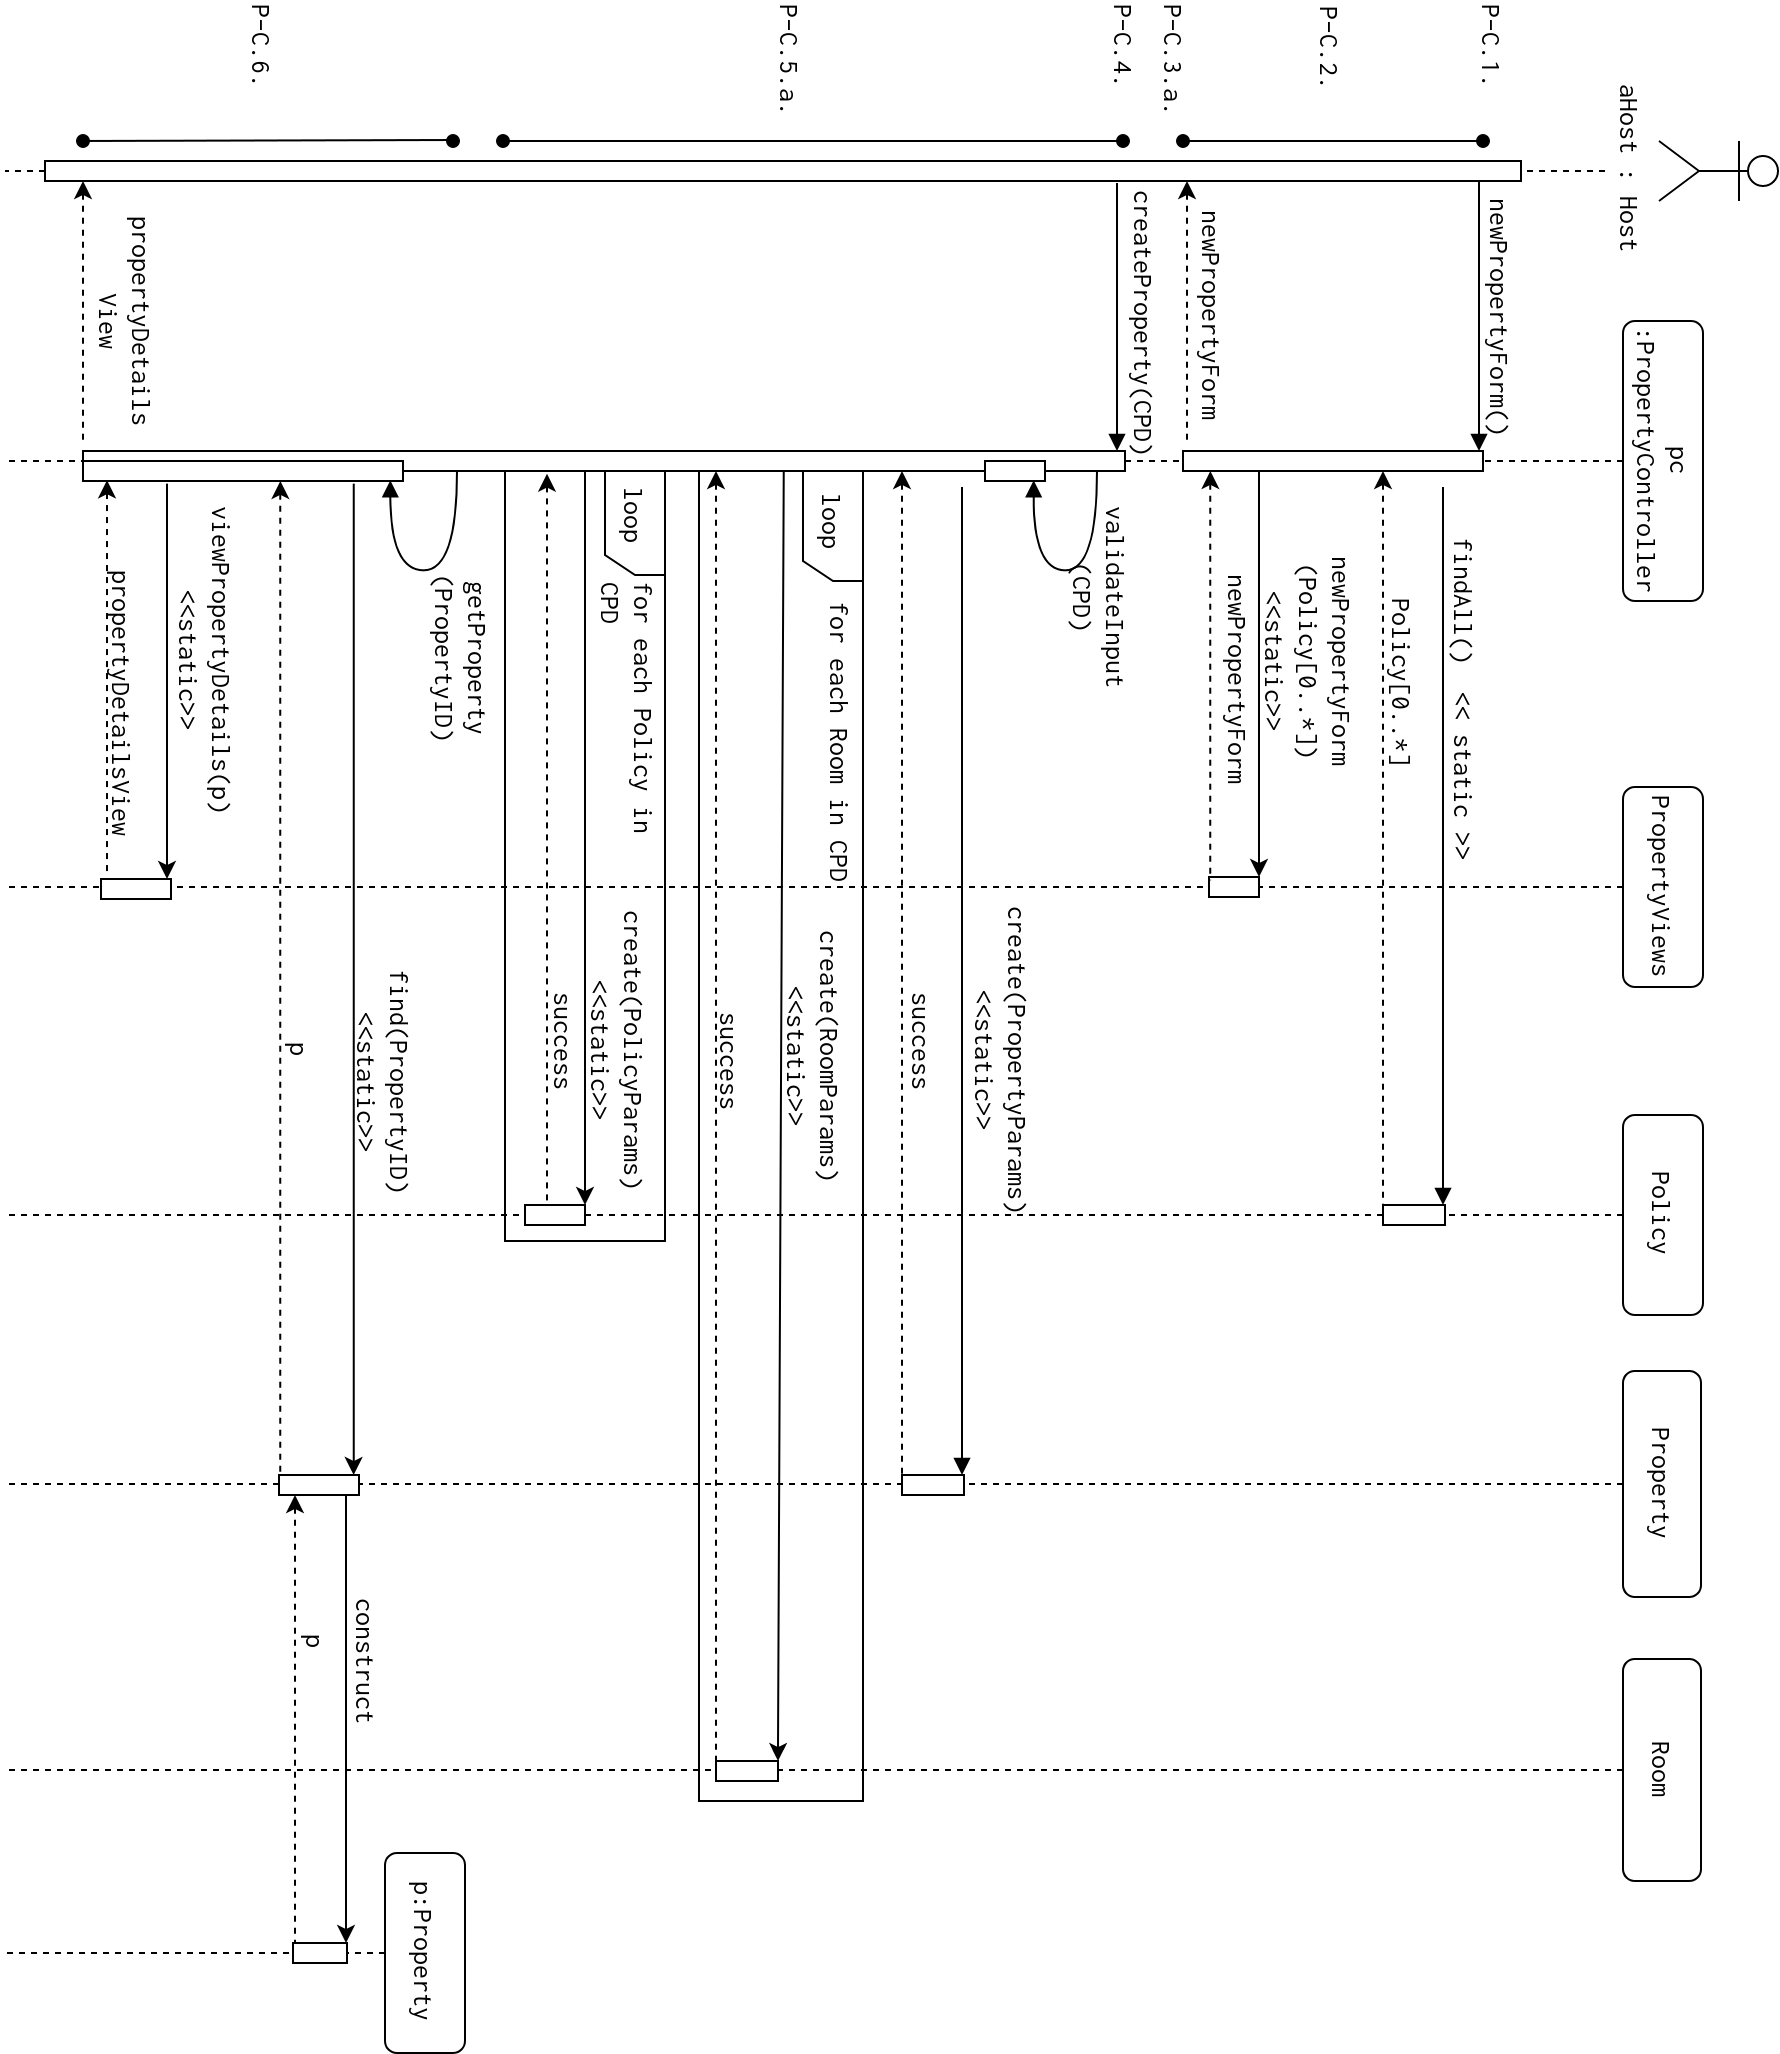
\includegraphics[width=16cm]{img/seq_diagrams/sqd_p_c.png} \\[0.5em]
    \caption{Sequence Diagram: Register Property}
    \label{Sequence Diagram: Register Property}
\end{figure} 

\begin{figure}[H]
    \centering
    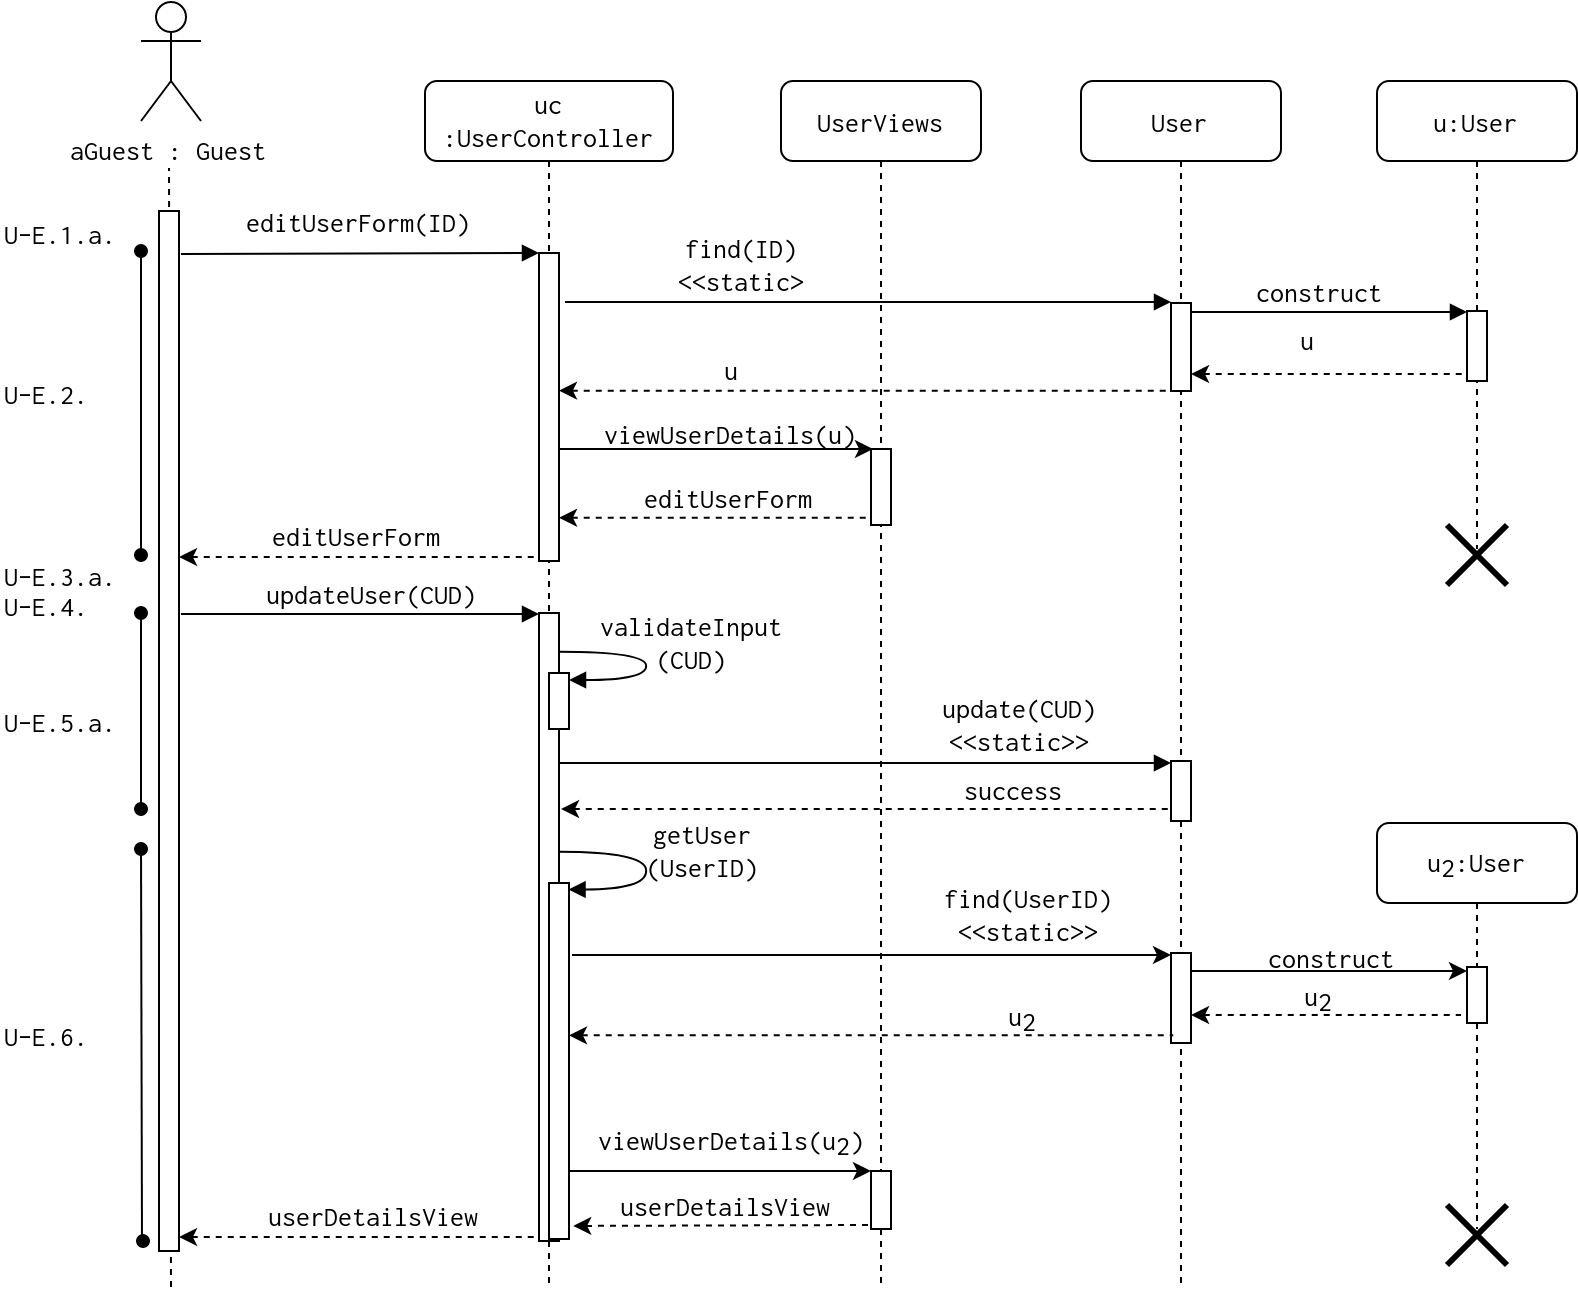
\includegraphics[width=13cm]{img/seq_diagrams/sqd_e_u.png} \\[0.5em]
    \caption{Sequence Diagram: Edit User}
    \label{Sequence Diagram: Edit User}
\end{figure}

\begin{figure}[H]
    \centering
    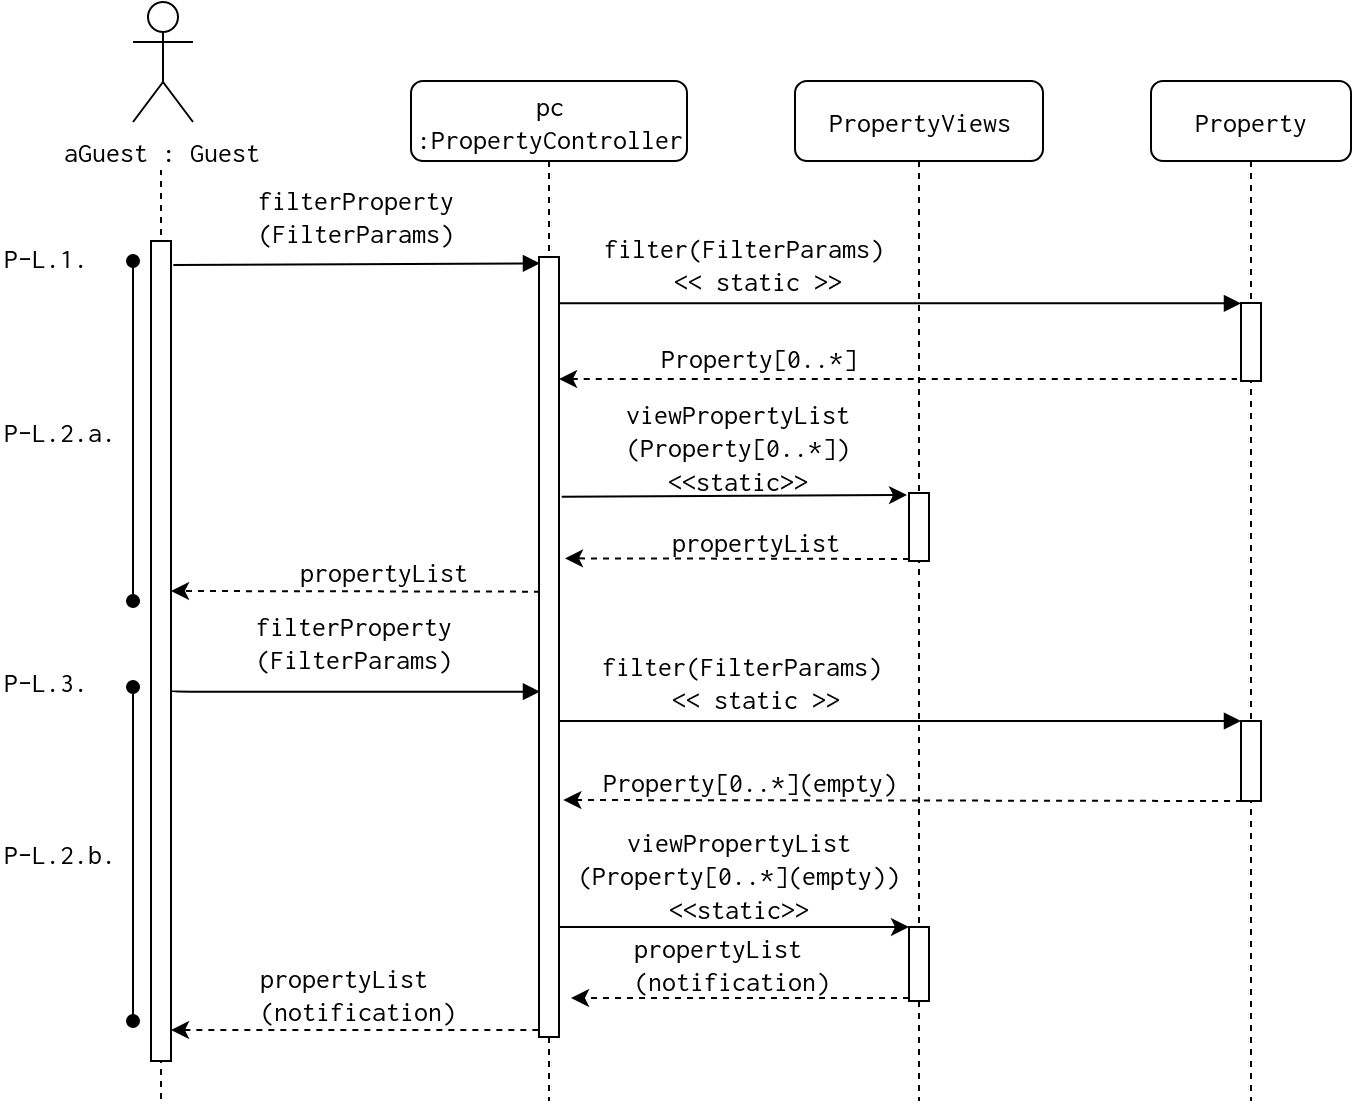
\includegraphics[width=13cm]{img/seq_diagrams/sqd_p_l.png} \\[0.5em]
    \caption{Sequence Diagram: View Property List}
    \label{Sequence Diagram: View Property List}
\end{figure}

\begin{figure}[H]
    \centering
    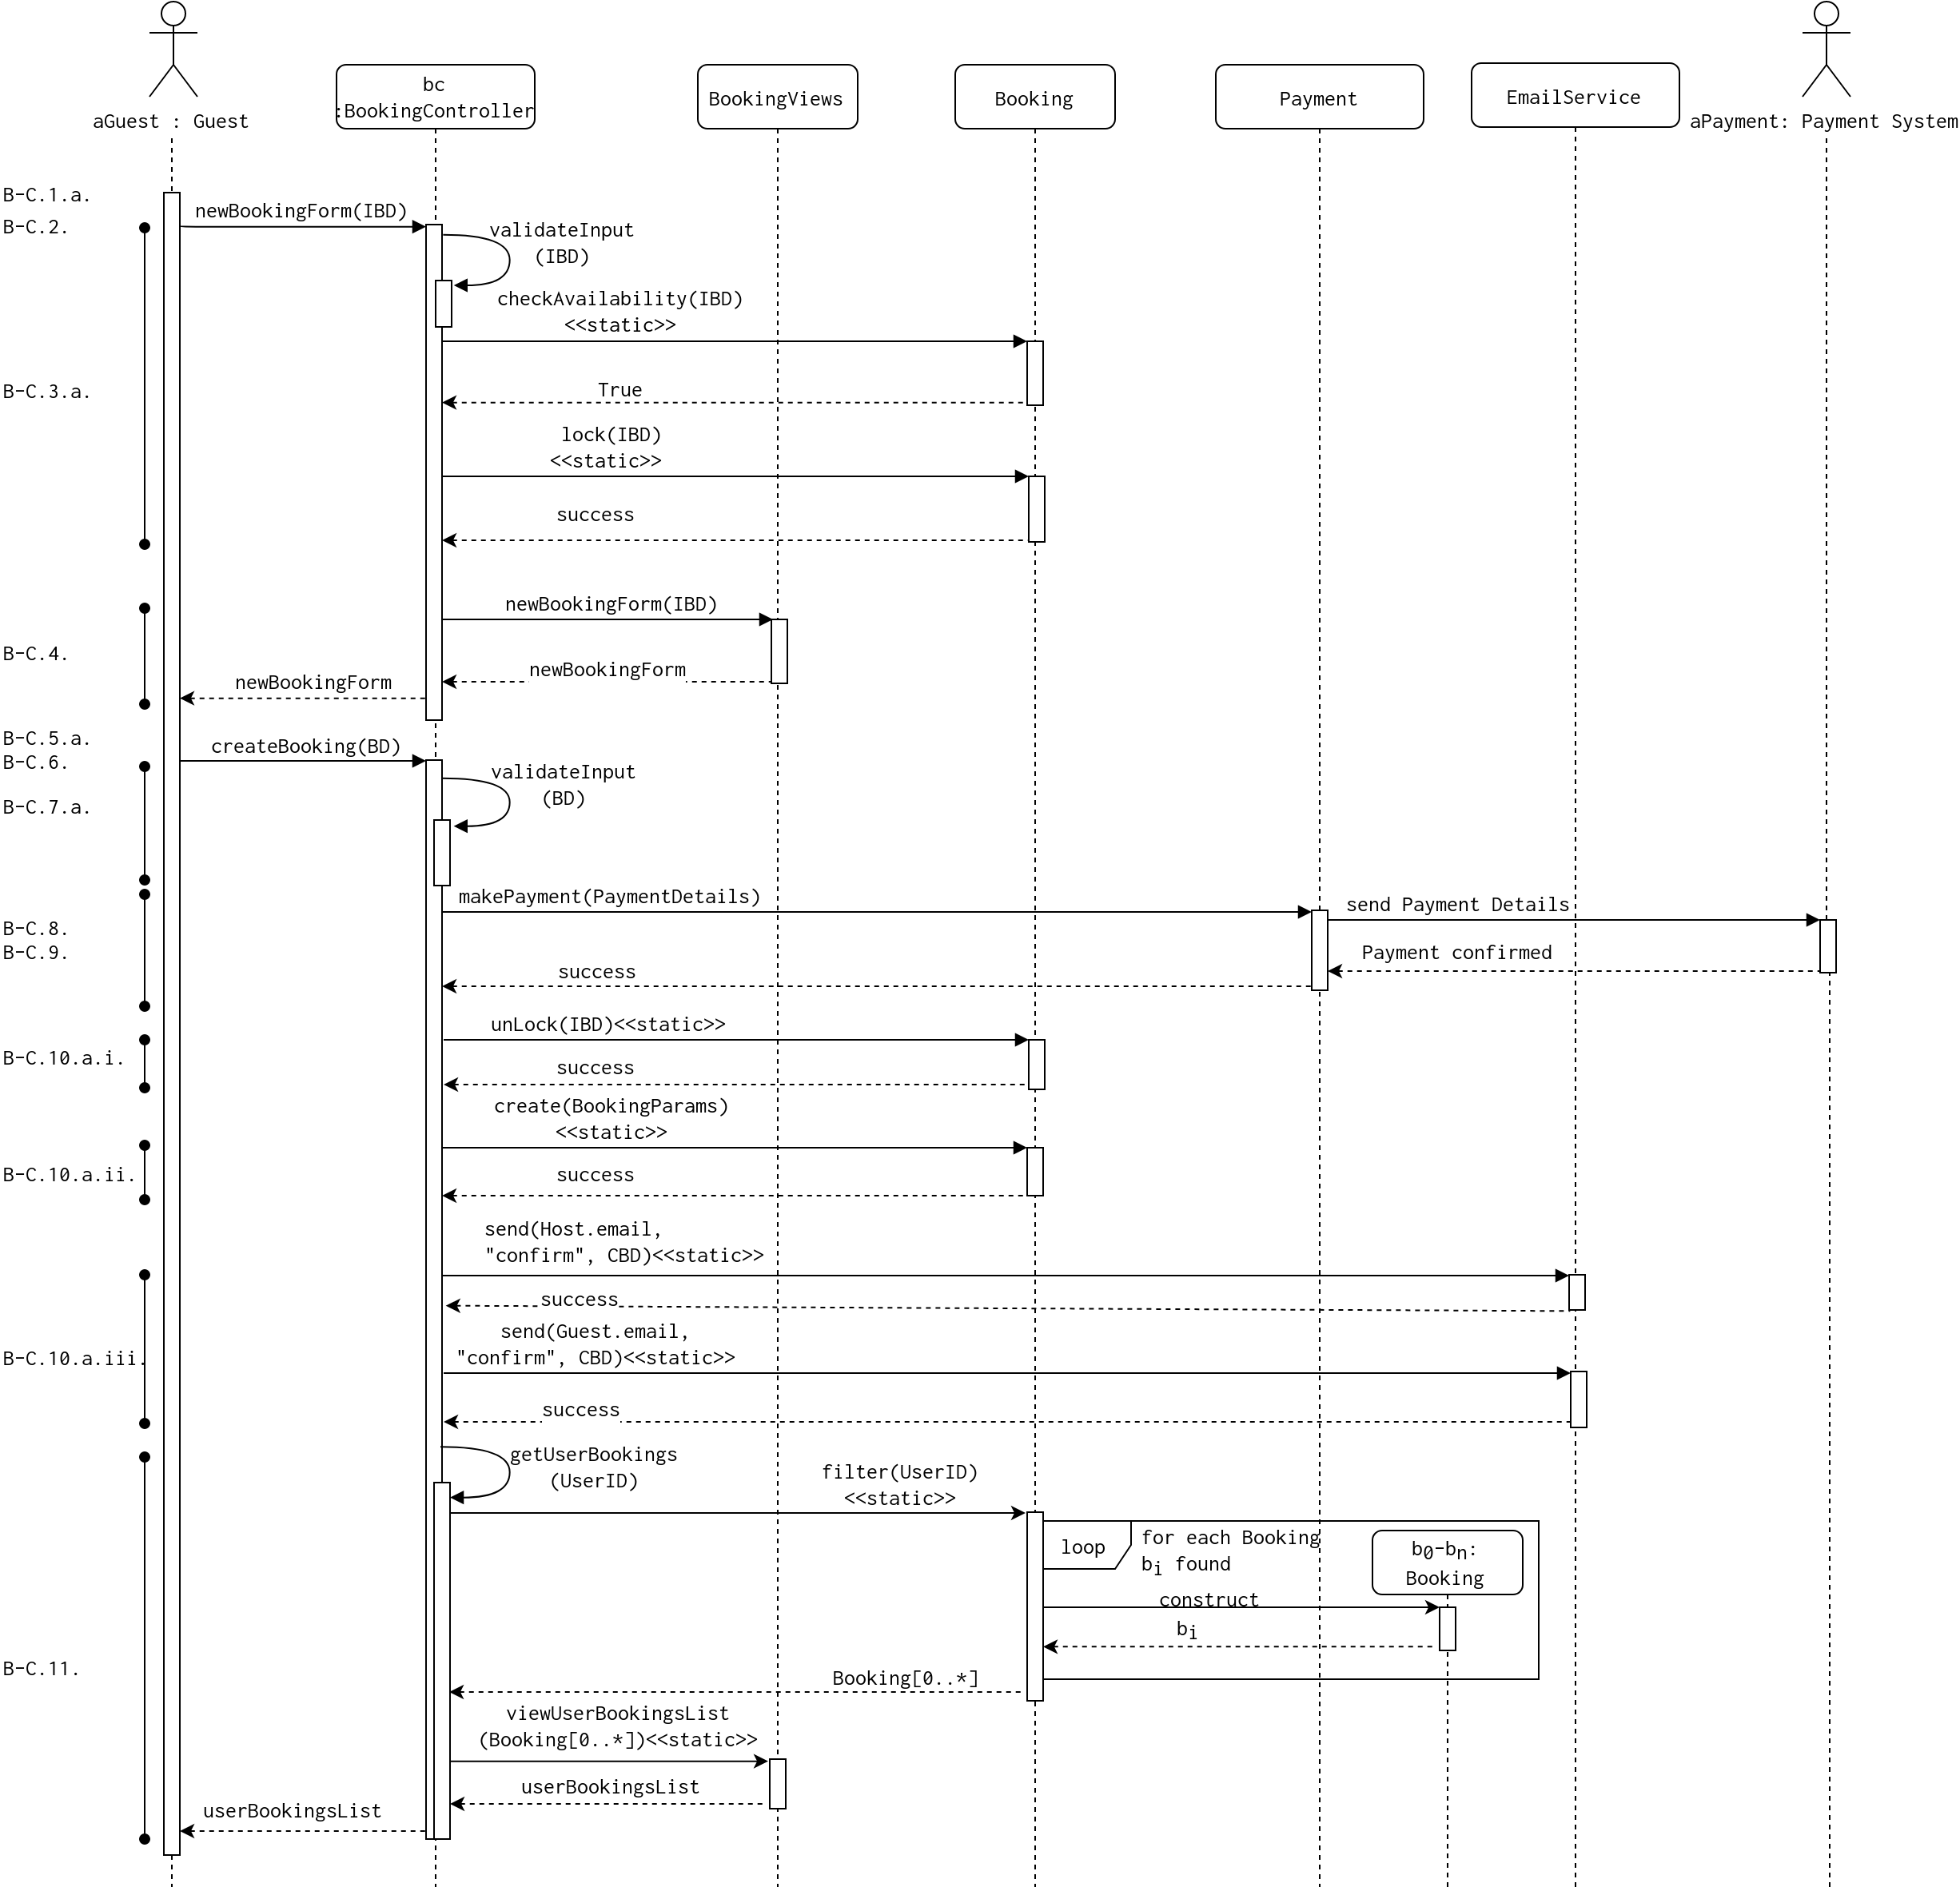
\includegraphics[width=\textwidth]{img/seq_diagrams/sqd_b_c.png} \\[0.5em]
    \caption{Sequence Diagram: Make Booking}
    \label{Sequence Diagram: Make Booking}
\end{figure}

\begin{figure}[H]
    \centering
    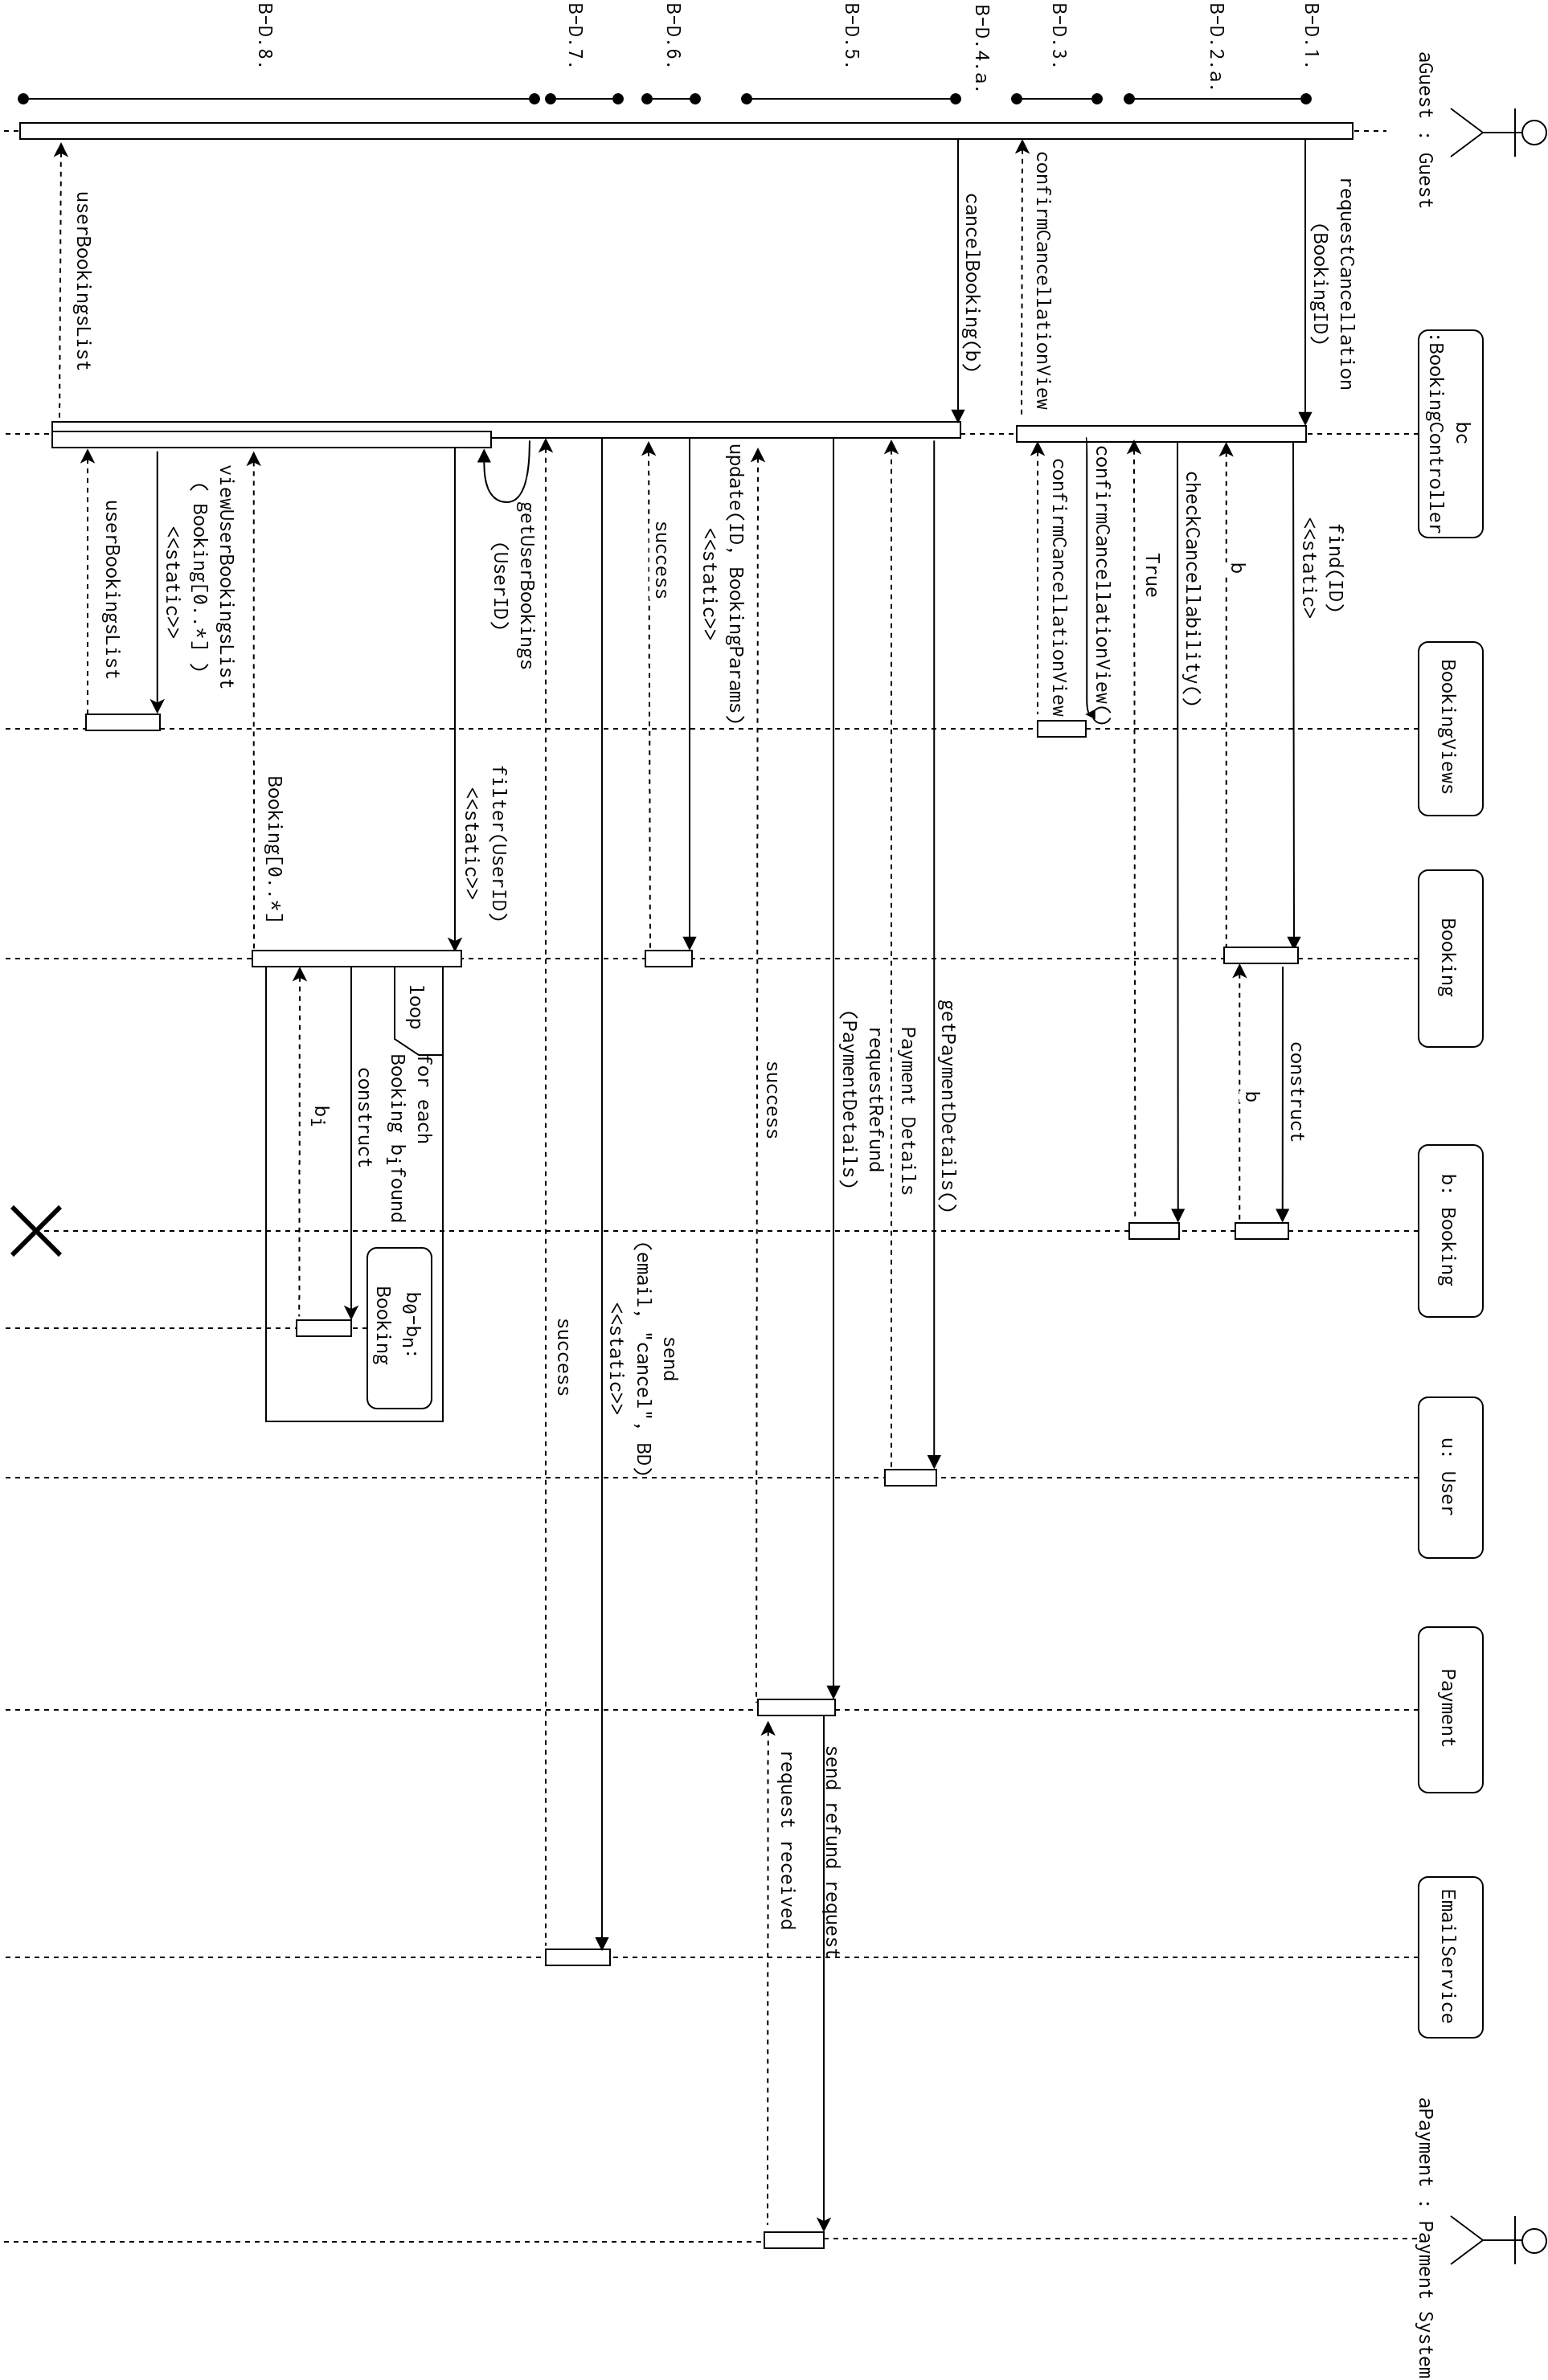
\includegraphics[width=16cm]{img/seq_diagrams/sqd_b_d.png} \\[0.5em]
    \caption{Sequence Diagram: Cancel Booking}
    \label{Sequence Diagram: Cancel Booking}
\end{figure}

\begin{figure}[H]
    \centering
    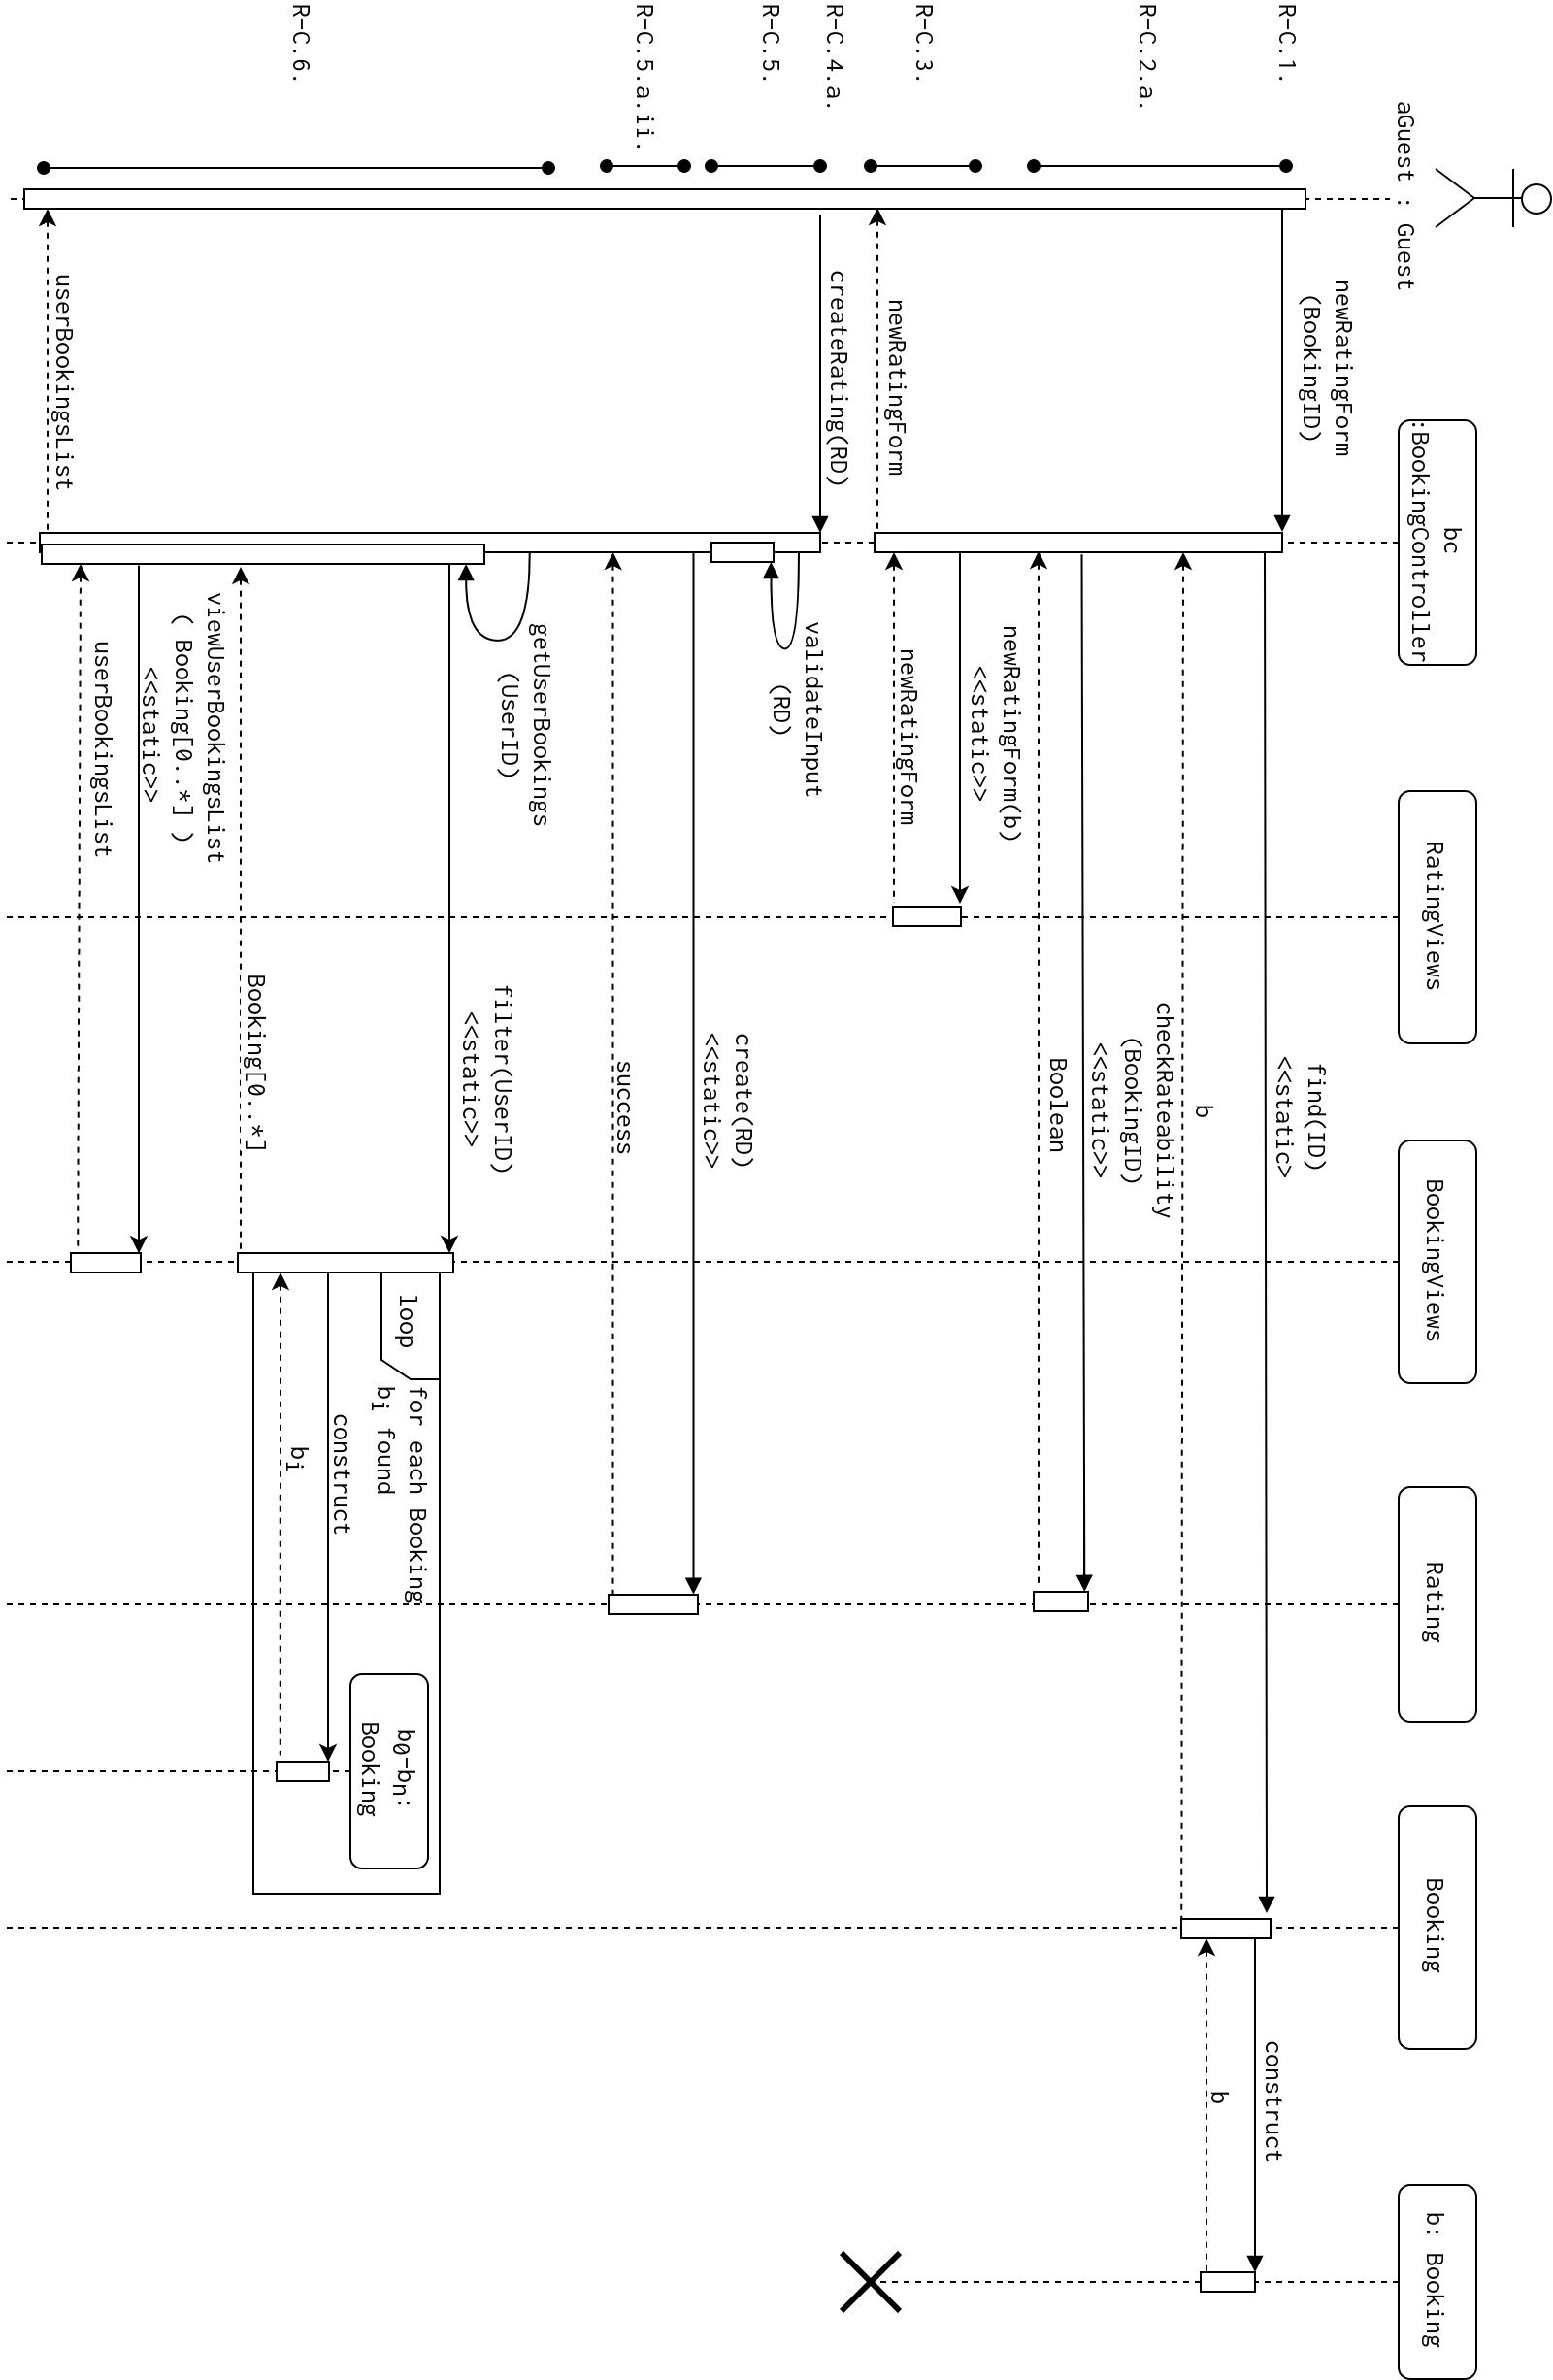
\includegraphics[width=16cm]{img/seq_diagrams/sqd_r_c.png} \\[0.5em]
    \caption{Sequence Diagram: Give Rating}
    \label{Sequence Diagram: Give Rating}
\end{figure}

% ==============================================================================
%                              STATE MACHINE DIAGRAM SECTION 
% ==============================================================================
\section{State Machine Diagram}\label{statemachine_section}

A state machine diagram is a type of behavioural diagram that shows transitions between various objects. Based on the input it receives it can change its status and thereby determine which operations an object can perform at a given moment. The case depicted in the following figure shows the process by which a Guest makes a Booking. In the "Check property availability" composite state, the system checks the property for availability in a few different sub-states. If the time is not available on the room, the process will be escaped. If the room shows availability, however, the booking will be added. To transition from available to unavailable, a booking for this property is created. To exit the unavailable state, a booking is either deleted or lies in the past.

\begin{figure}[H]
    \centering
    \label{state_machine_diagram}
    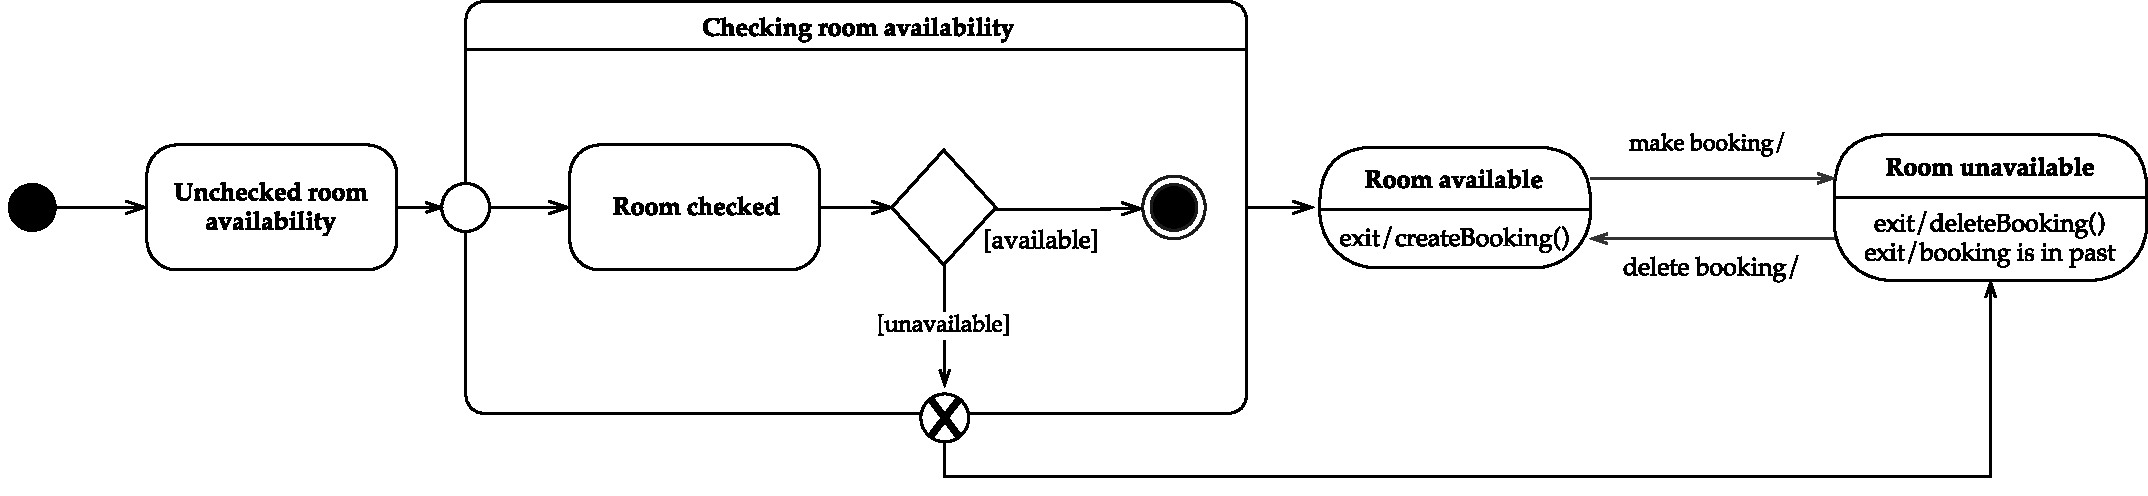
\includegraphics[width=\textwidth]{img/state_machine_diagram.pdf}
    \caption{State Machine Diagram: Make booking}
\end{figure}


% ==============================================================================
%                              ACTIVITY DIAGRAM SECTION 
% ==============================================================================
\section{Activity View}

Following the design flow from the static view on the system (cf. Figure \ref{design_diagram}) to the interaction view in the form of sequence diagrams (cf. section \ref{sequence_section}), this section aims to show the control flow in the system in a more abstract way via the activity view. UML activity diagrams present business processes executed by users interacting with the system.

Figures \ref{activity_diagram_1} -- \ref{activity_diagram_4} describe in more detail how the use cases detailed in chapter \ref{chapter:use cases} translate into a sequence forming main business processes. An overview of which use cases map to a specific activity is given in Figure \ref{activity-use case-mapping}\footnote{The colour code in the \textquotesingle ID \textquotesingle column refers to the Actor involved in the activity, rather than the Actor set that is generally eligible for the use case.}. As the final product aims at matching Property hosts with potential Property guests, activities such as the Guest making a Booking, Host registering a Property or cancelling a Booking are selected as primary examples.

Activity diagrams are useful in identifying and specifying the sequential and concurrent nature of dependencies in the system. Whereas the sequence diagrams show the control flow between objects and hence show the technical implementation of a use case depicting operations on classes and message interaction, the activity diagrams below give a high-level overview of the execution behaviour of the system and do not show objects that perform the activities \cite{UMLReference2004}. Note how different types of control nodes specify the sequencing of action nodes and the high-level description of validation processes that are inherited in the behaviour of decision nodes \cite{UML2017}.
Refer to the User Manual in section \ref{chapter:mockups} on how the control described in this section translates into the user interface.

\begin{table}[H]
    \centering
    \begin{tabular}{| p{3cm} | p{1.25cm} | p{11cm} |}
        \hline
        Activity & ID                 & Use Case                \\ \hline \hline
                    & \cellcolor{V}U-C-1 & \thead{A Visitor registers as a Guest or a Host.} \\ \cline{2-3}
                    \multirow{-2}{*}{\thead{Host \& Property \\ Registration}}
                    & \cellcolor{H}P-C   & \thead{A Host registers a new Property.} \\
        \hline
& \cellcolor{G}F-L & \thead{A Guest views their Favourites.} \\ \cline{2-3}
                    & \cellcolor{G}P-V   & \thead{A Guest, Admin, or a Host views a Property\textquotesingle s Property
Details.} \\ \cline{2-3}
        \multirow{-3}{*}{\thead{Guest make \\ Booking}}
                    & \cellcolor{G}B-C   & \thead{The Guest makes a new Booking.} \\ \hline
                    & \cellcolor{G}P-L & \thead{A Guest or an Admin searches for, filters, orders, \\ and views a List of Properties.} \\ \cline{2-3}
                    & \cellcolor{G}F-C   & \thead{A Guest adds a Property to their Favourites.} \\ \cline{2-3}
        \multirow{-3}{*}{\thead{Guest search \\ Properties}}
                    & \cellcolor{G}F-D   & \thead{A Guest removes a Property from their Favourites.} \\ \hline
                    & \cellcolor{H}B-L-2 & \thead{A Host views their own Property\textquotesingle s Bookings, \\ or an Admin views any Property\textquotesingle s
Bookings.} \\ \cline{2-3}\multirow{-2}{*}{\thead{Host cancel  \\ Booking}} 
                    & \cellcolor{H}B-D   & \thead{A Guest cancels one of their own Cancellable Bookings,\\ or a Host cancels
a Cancellable Booking on their Property.} \\ \cline{2-3} \hline
    \end{tabular}
    \caption{Activity \& Use Case Mapping}
    \label{activity-use case-mapping}
\end{table}
        
\begin{figure}[H]
    \centering
    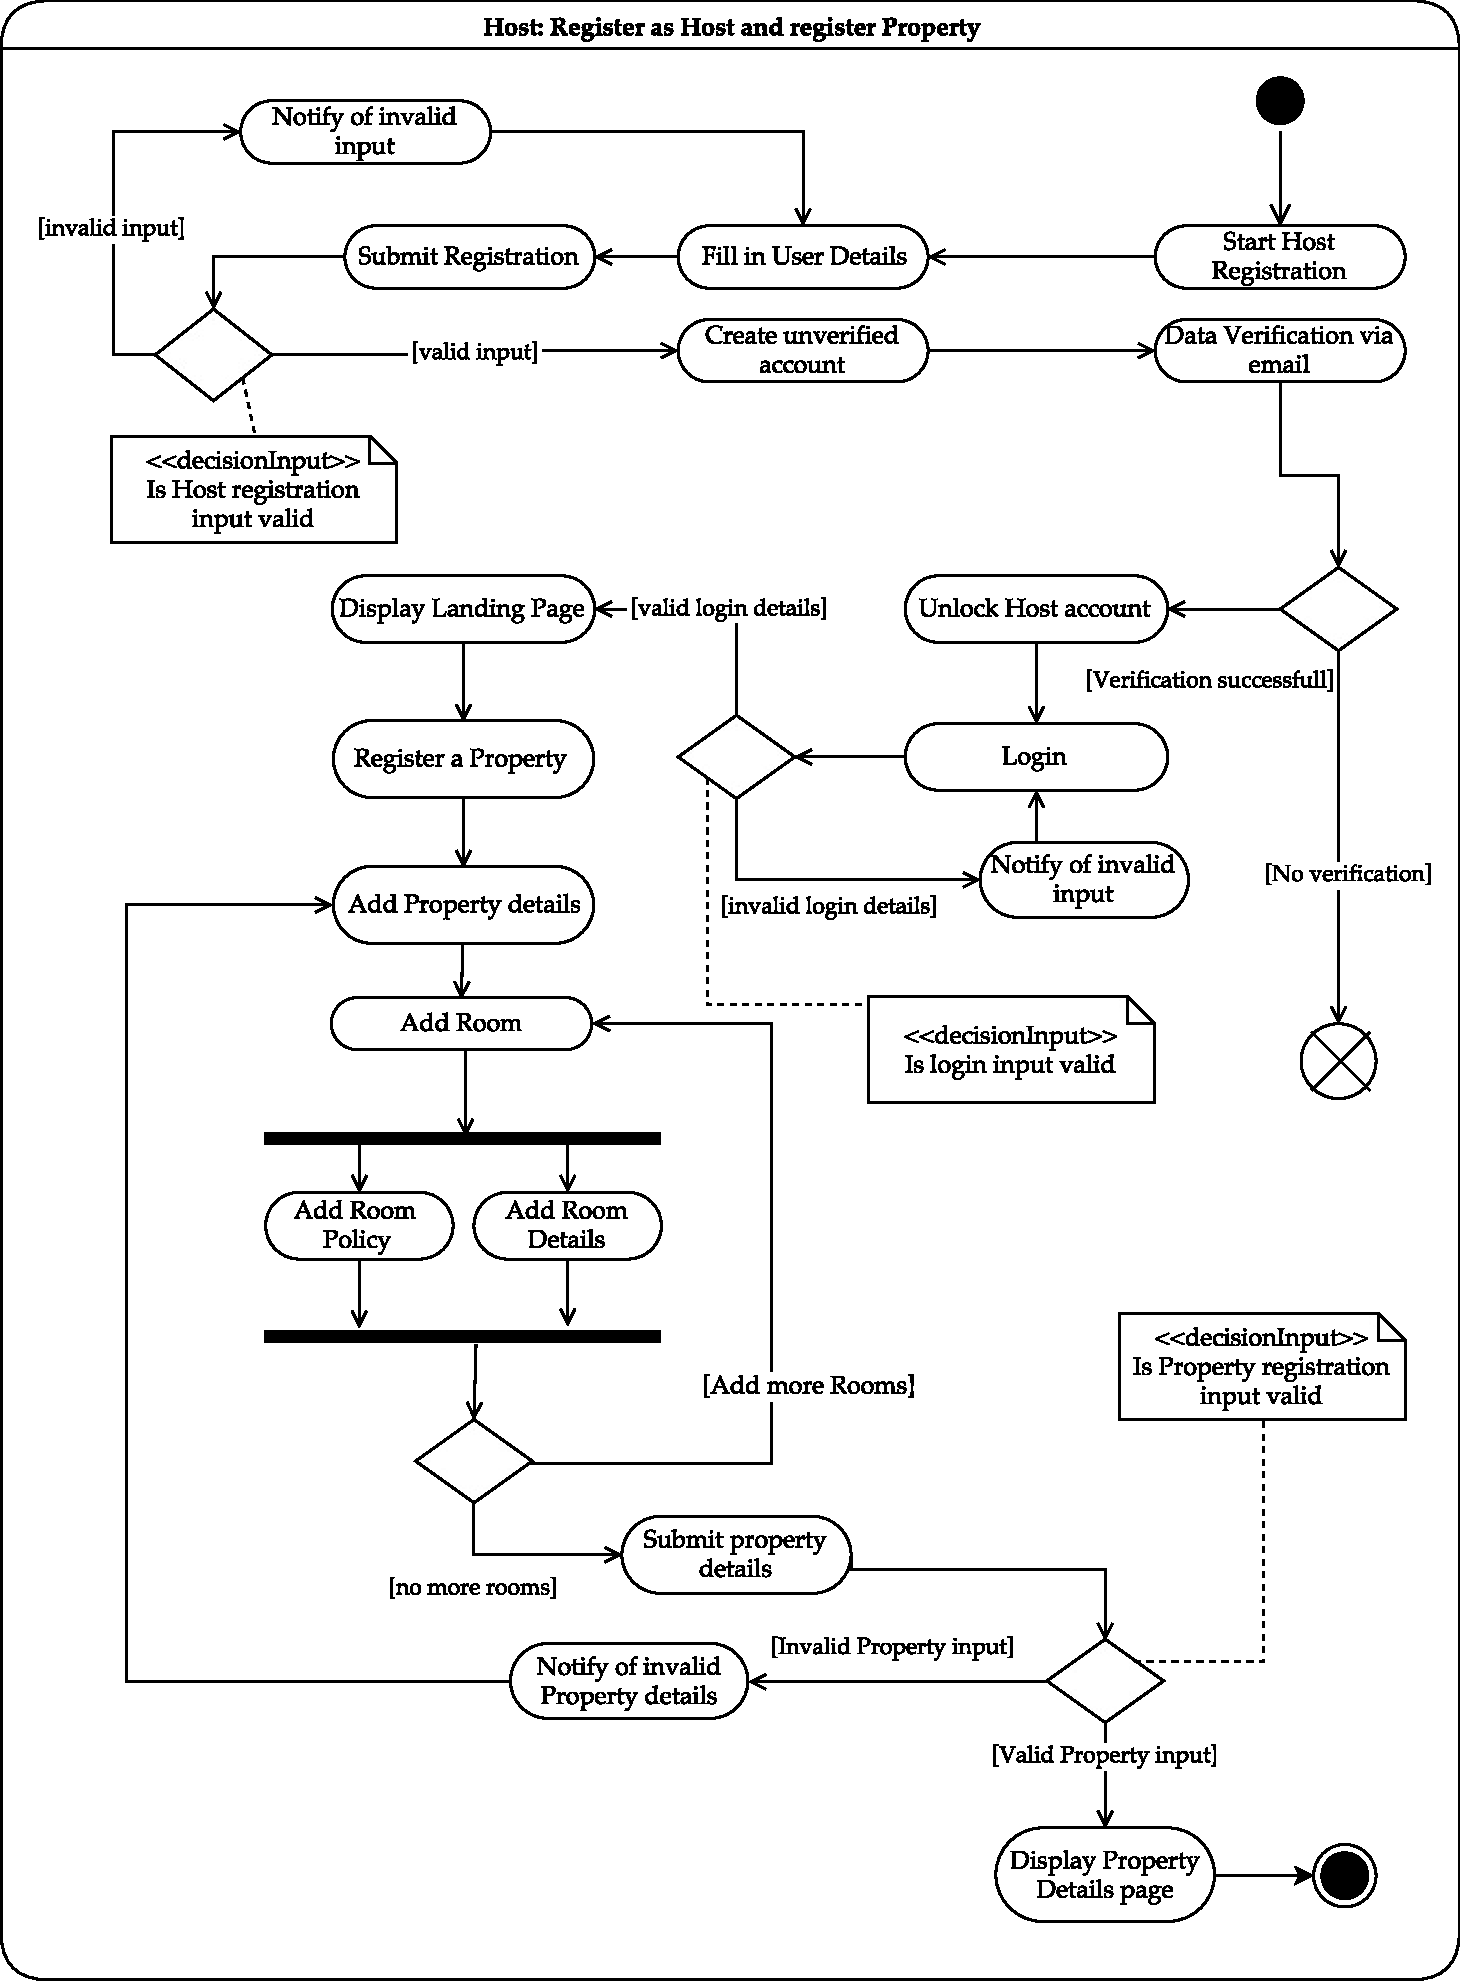
\includegraphics[width=17cm]{img/activity/register_property.pdf}
    \caption{Activity Diagram: Host \& Property Registration}
    \label{activity_diagram_1}
\end{figure}

\begin{figure}[H]
    \centering
    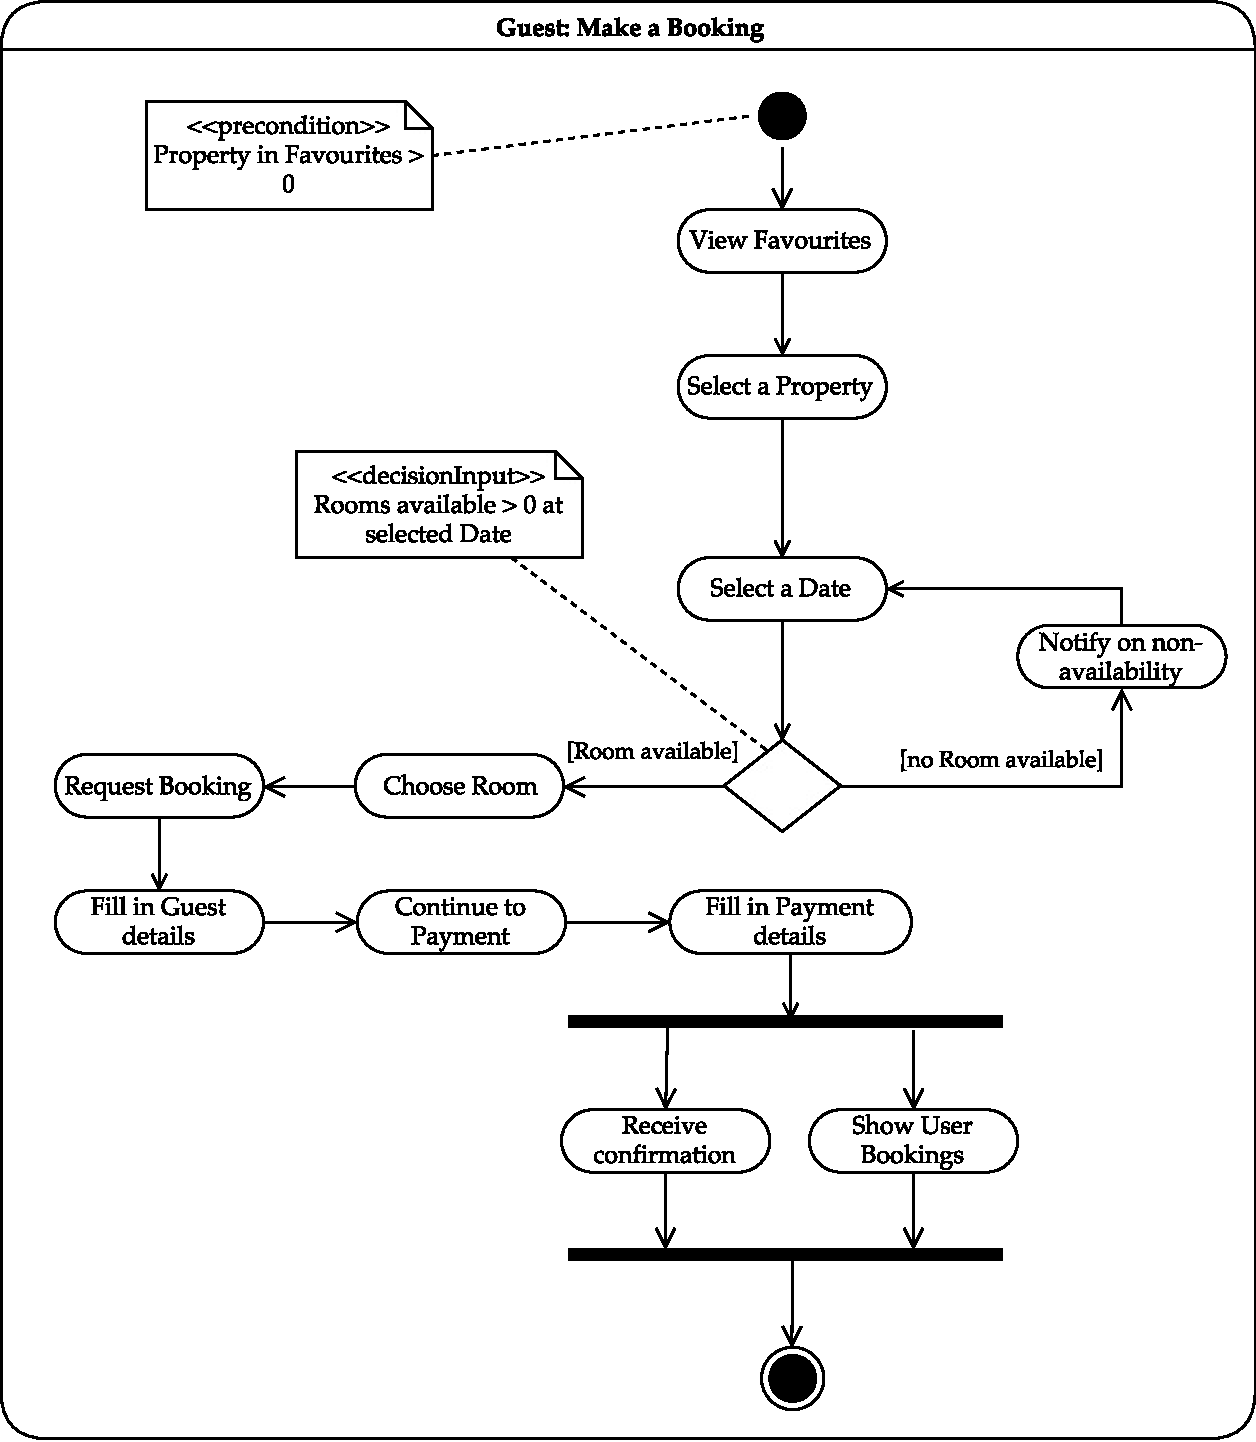
\includegraphics[width=17cm]{img/activity/make_booking.pdf}
    \caption{Activity Diagram: Guest Booking}
    \label{activity_diagram_2}
\end{figure}

\begin{figure}[H]
    \centering
    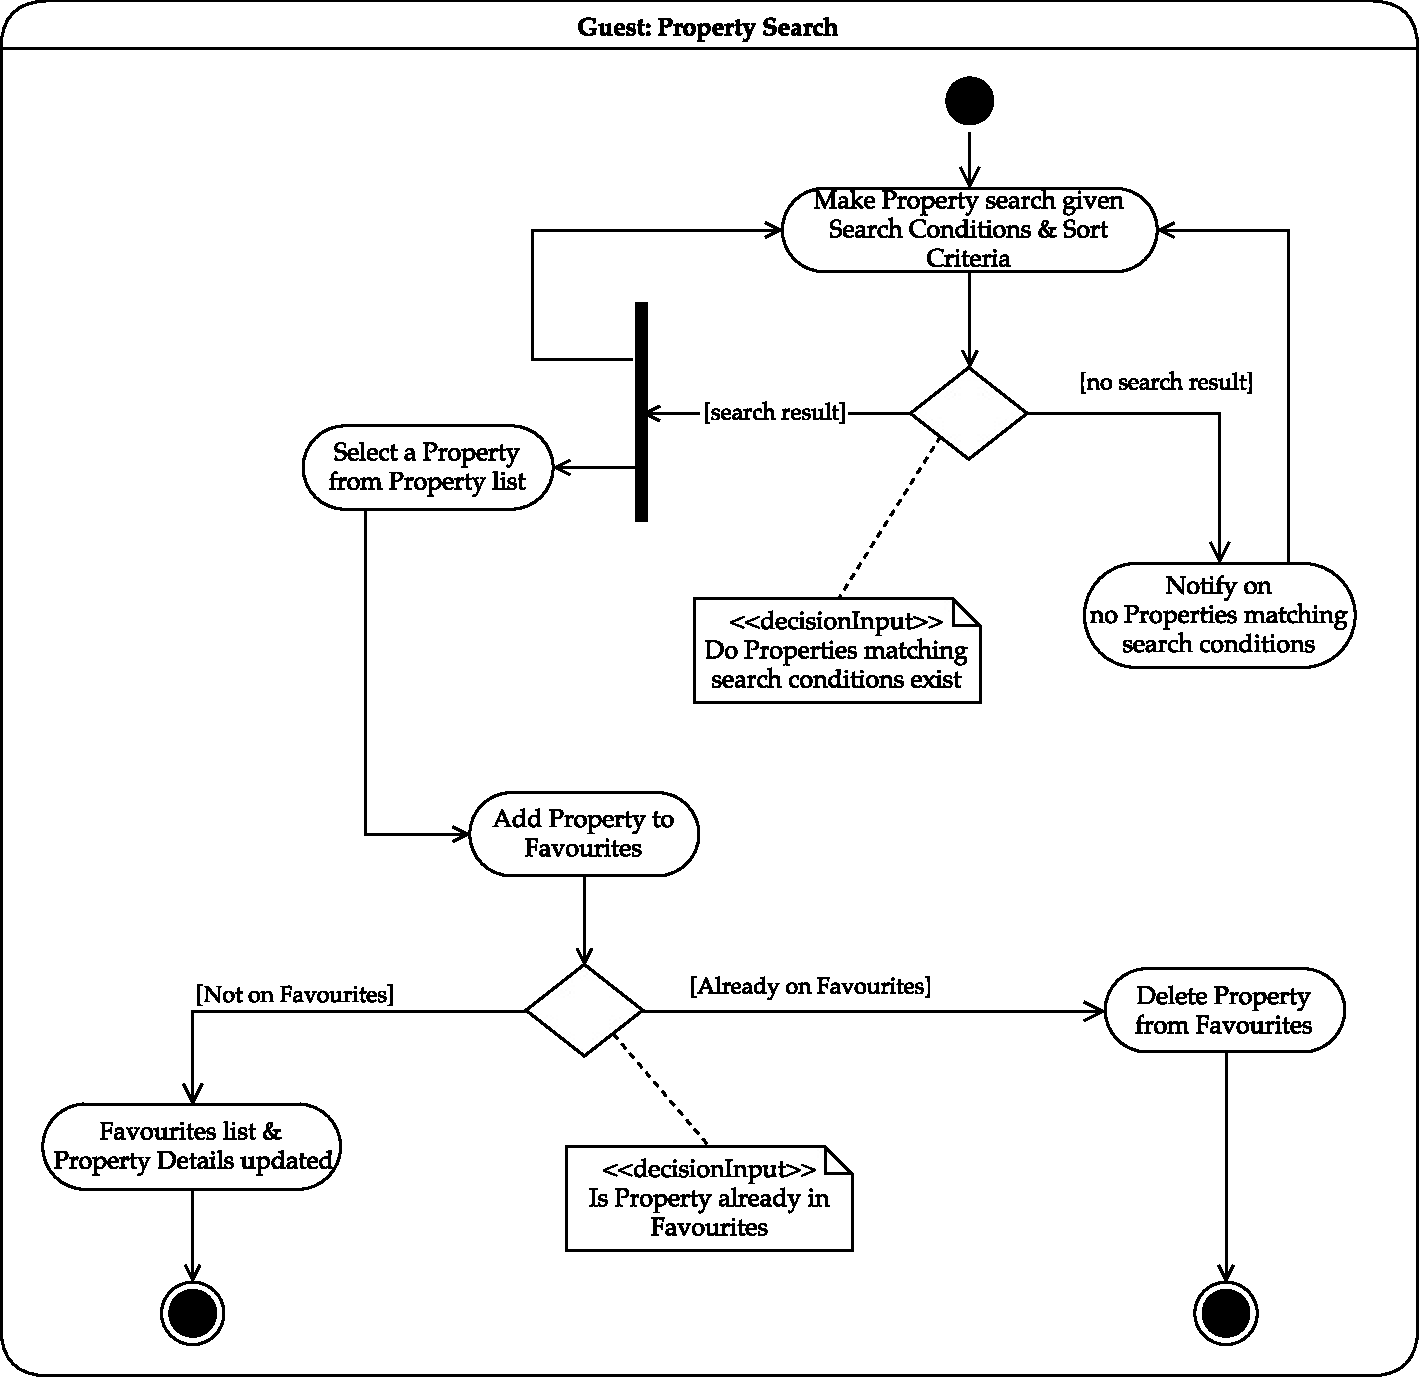
\includegraphics[width=17cm]{img/activity/search.pdf}
    \caption{Activity Diagram: Search Properties\protect\footnotemark}
    \label{activity_diagram_3}
\end{figure}
\footnotetext{The action node for selecting a Property implies the view of the Property Details page}	
\begin{figure}[H]
    \centering
    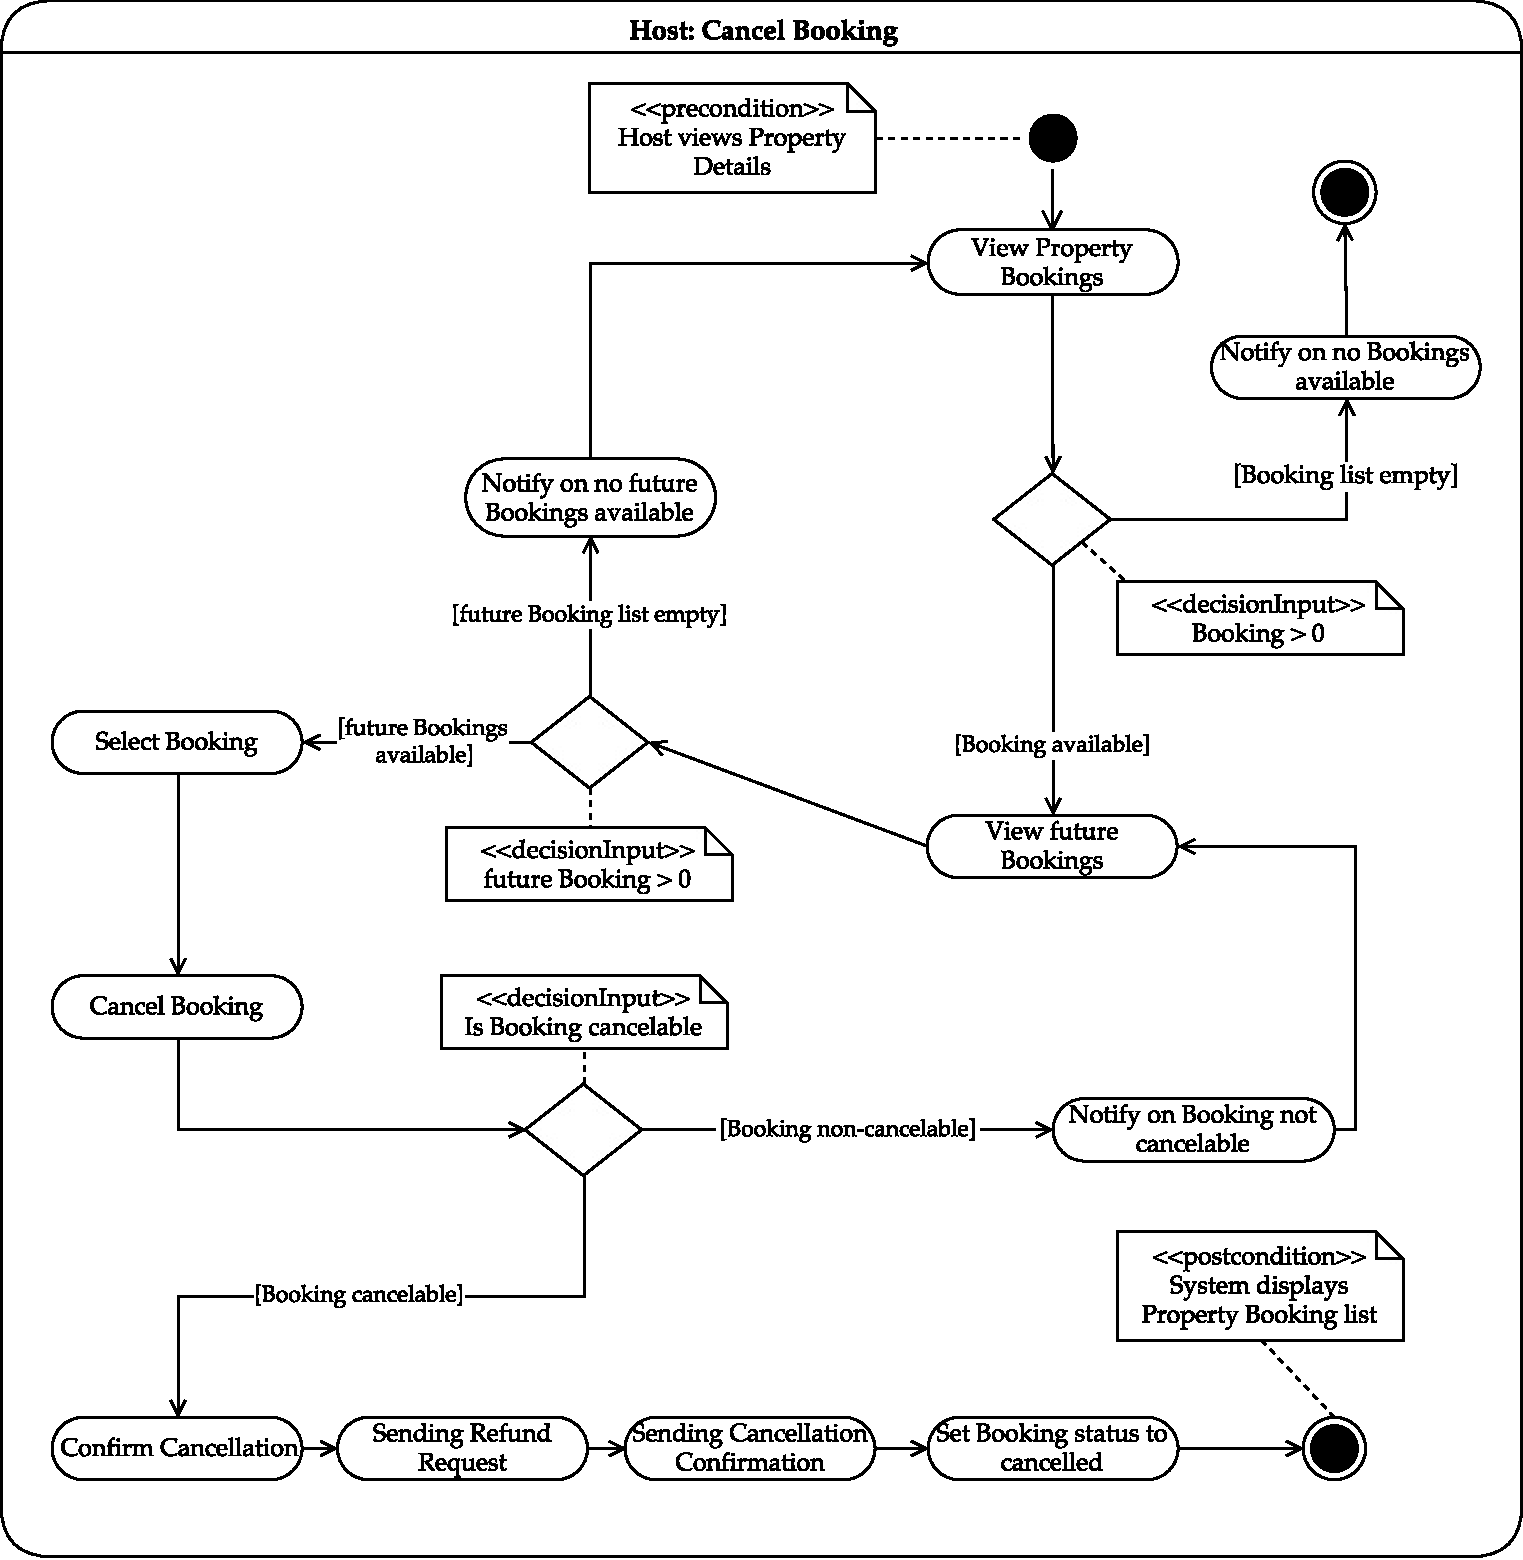
\includegraphics[width=17cm]{img/activity/cancel_booking.pdf}
    \caption{Activity Diagram: Host Cancel Booking}
    \label{activity_diagram_4}
\end{figure}

% ==============================================================================
%                              COMPONENT DIAGRAM SECTION 
% ==============================================================================
\section{Component Diagram}\label{component_section}
A generalised architectural overview of the entire system can be visualised using figure \ref{component_diagram}. Since components are parts of the system that are encapsulated, reusable, and replaceable \cite{Hamilton2006}, the component diagram shows how the usage of the widely adopted Model-View-Controller architectural pattern, usually referred to as MVC \cite{Fowler2006}, takes full advantage of these best practices.

The aforementioned diagram builds on the Design and Analysis diagrams by combining similar components together. Within the system, there are three main component groups: Views, Controllers, and Models. The classes under each group of components are responsible for a similar set of tasks. The View classes have the sole responsibility of generating strings from the inputs sent to them from the controllers. The strings will then be sent to the client browsers and effectively be rendered as HTML. The Controller classes are responsible for acting as a middle layer that talks to the Models and the Views. Controllers do not contain business logic but rather provide endpoints that can be called from the generated views. The Models group are the classes that contain the business logic and are directly connected to the database. 

\begin{figure}[H]
    \centering
    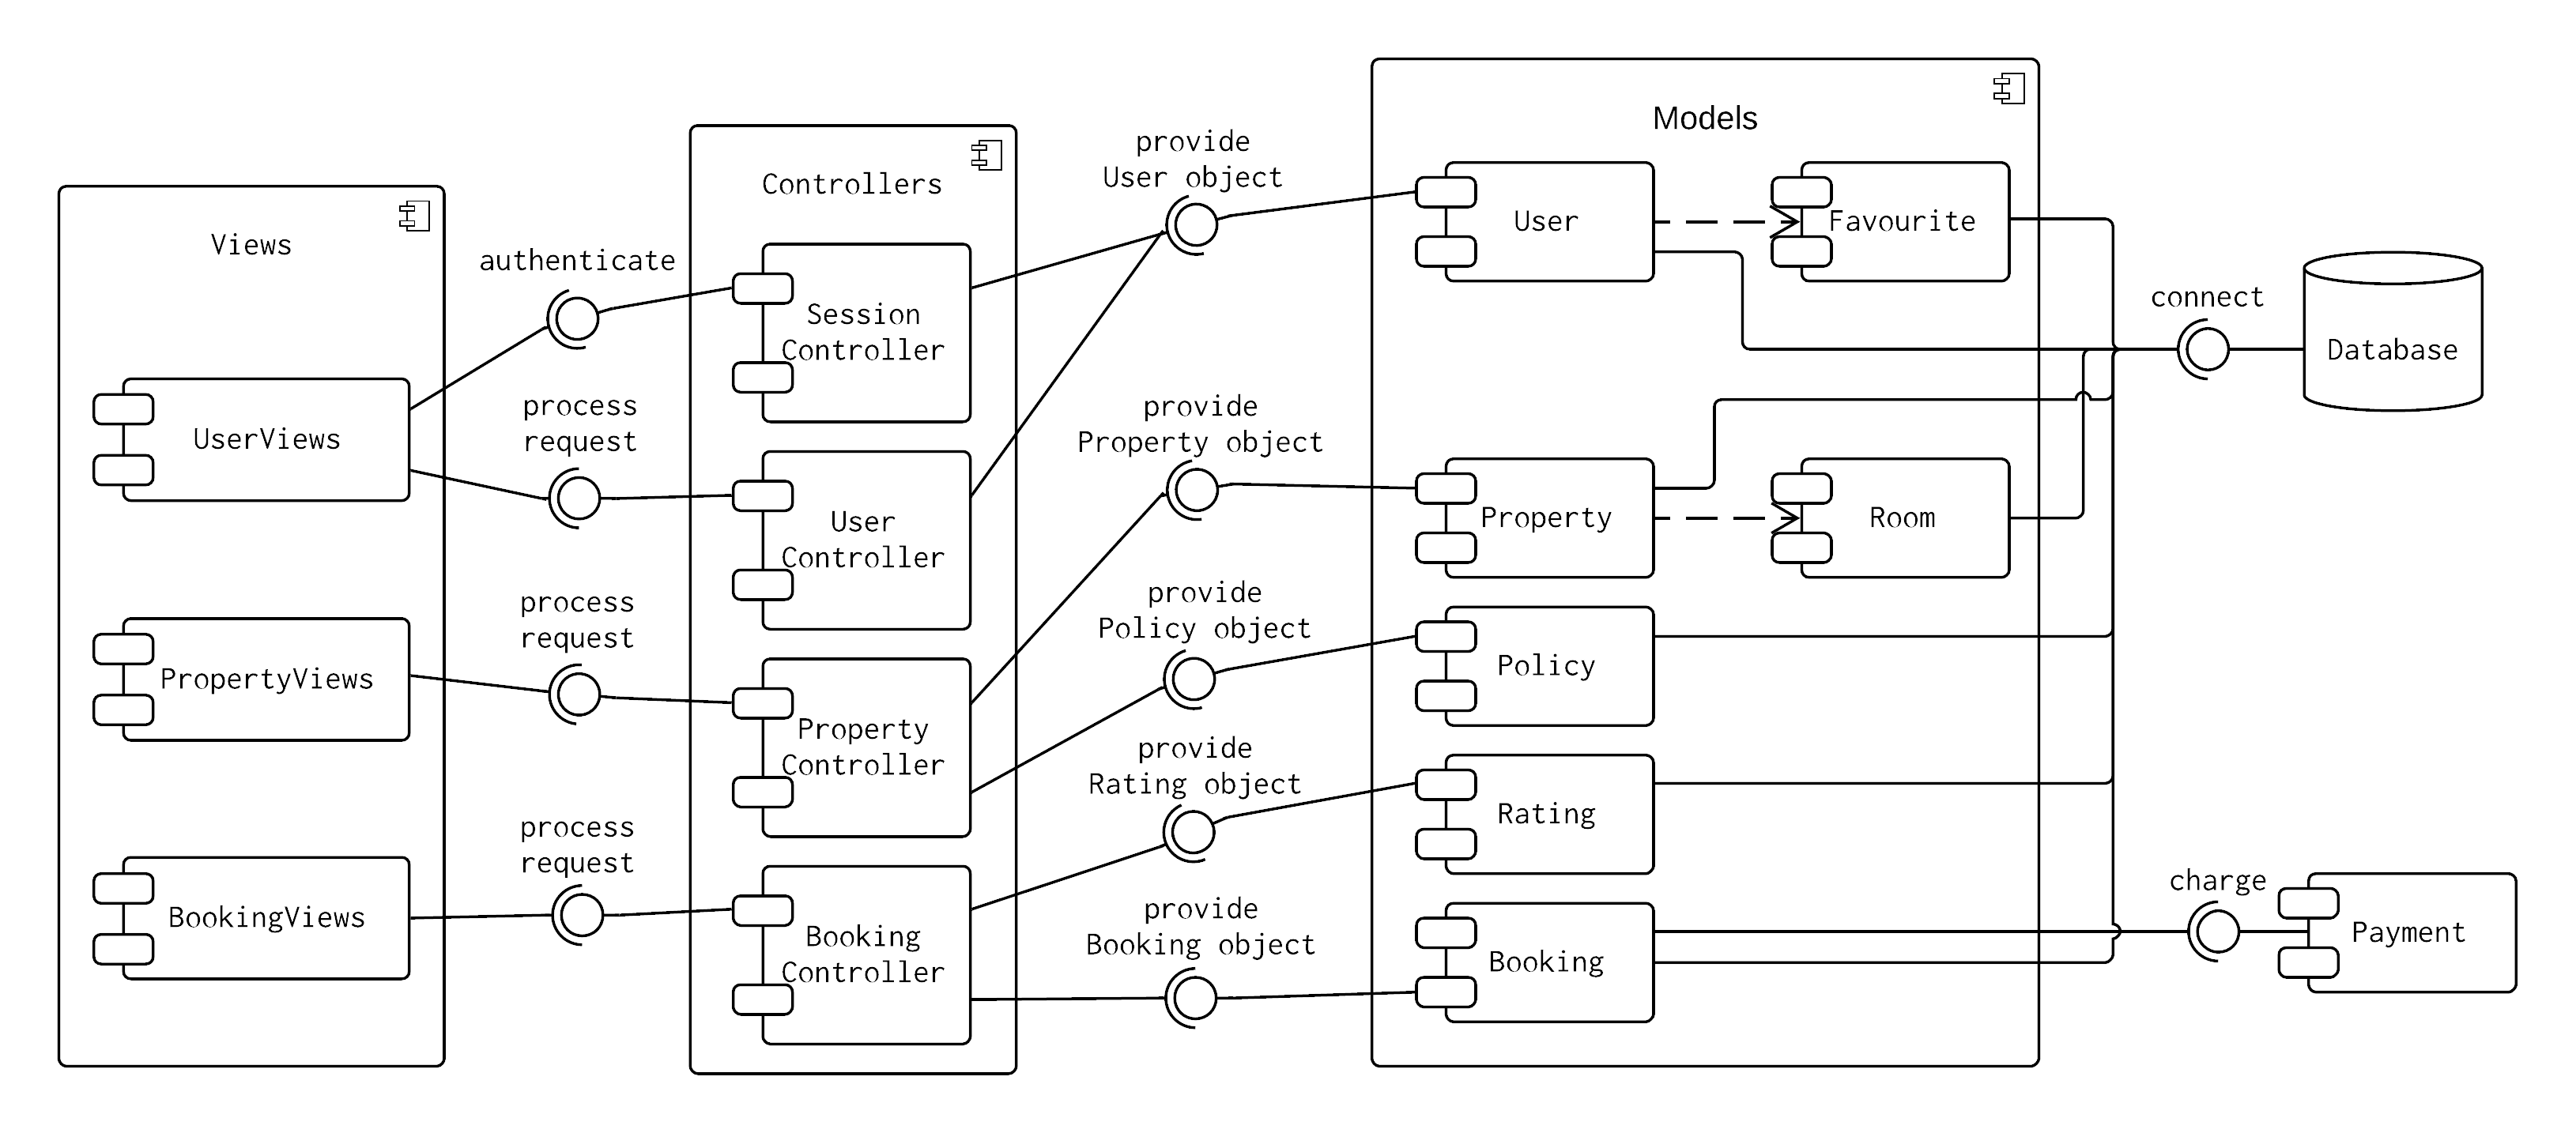
\includegraphics[width=\textwidth]{img/component_diagram.png}
    \caption{Component Diagram}
    \label{component_diagram}
\end{figure}

\section{Deployment Diagram}
The deployment to hardware environments is described using the following deployment diagram. This diagram shows the physical connections within the system in terms of deploying the software to a physical environment.

The system contains four main nodes:
\begin{itemize}
    \item \textit{UserClient} - A web browser such as Google Chrome, Safari, or Firefox that renders the HTML assets to the Users.
    \item \textit{WebServer} - Apache HTTP Server that will be responsible for dealing with HTTP requests and responses to/from clients.
    \item \textit{ApplicationServer} - A server such as Apache Tomcat which is capable of running Java EE specifications and hosts a suitable execution environment.
    \item \textit{DatabaseServer} - This server will be responsible for managing and maintaining MySQL Database that is connected to the system.
\end{itemize}

\begin{figure}[H]
    \centering
    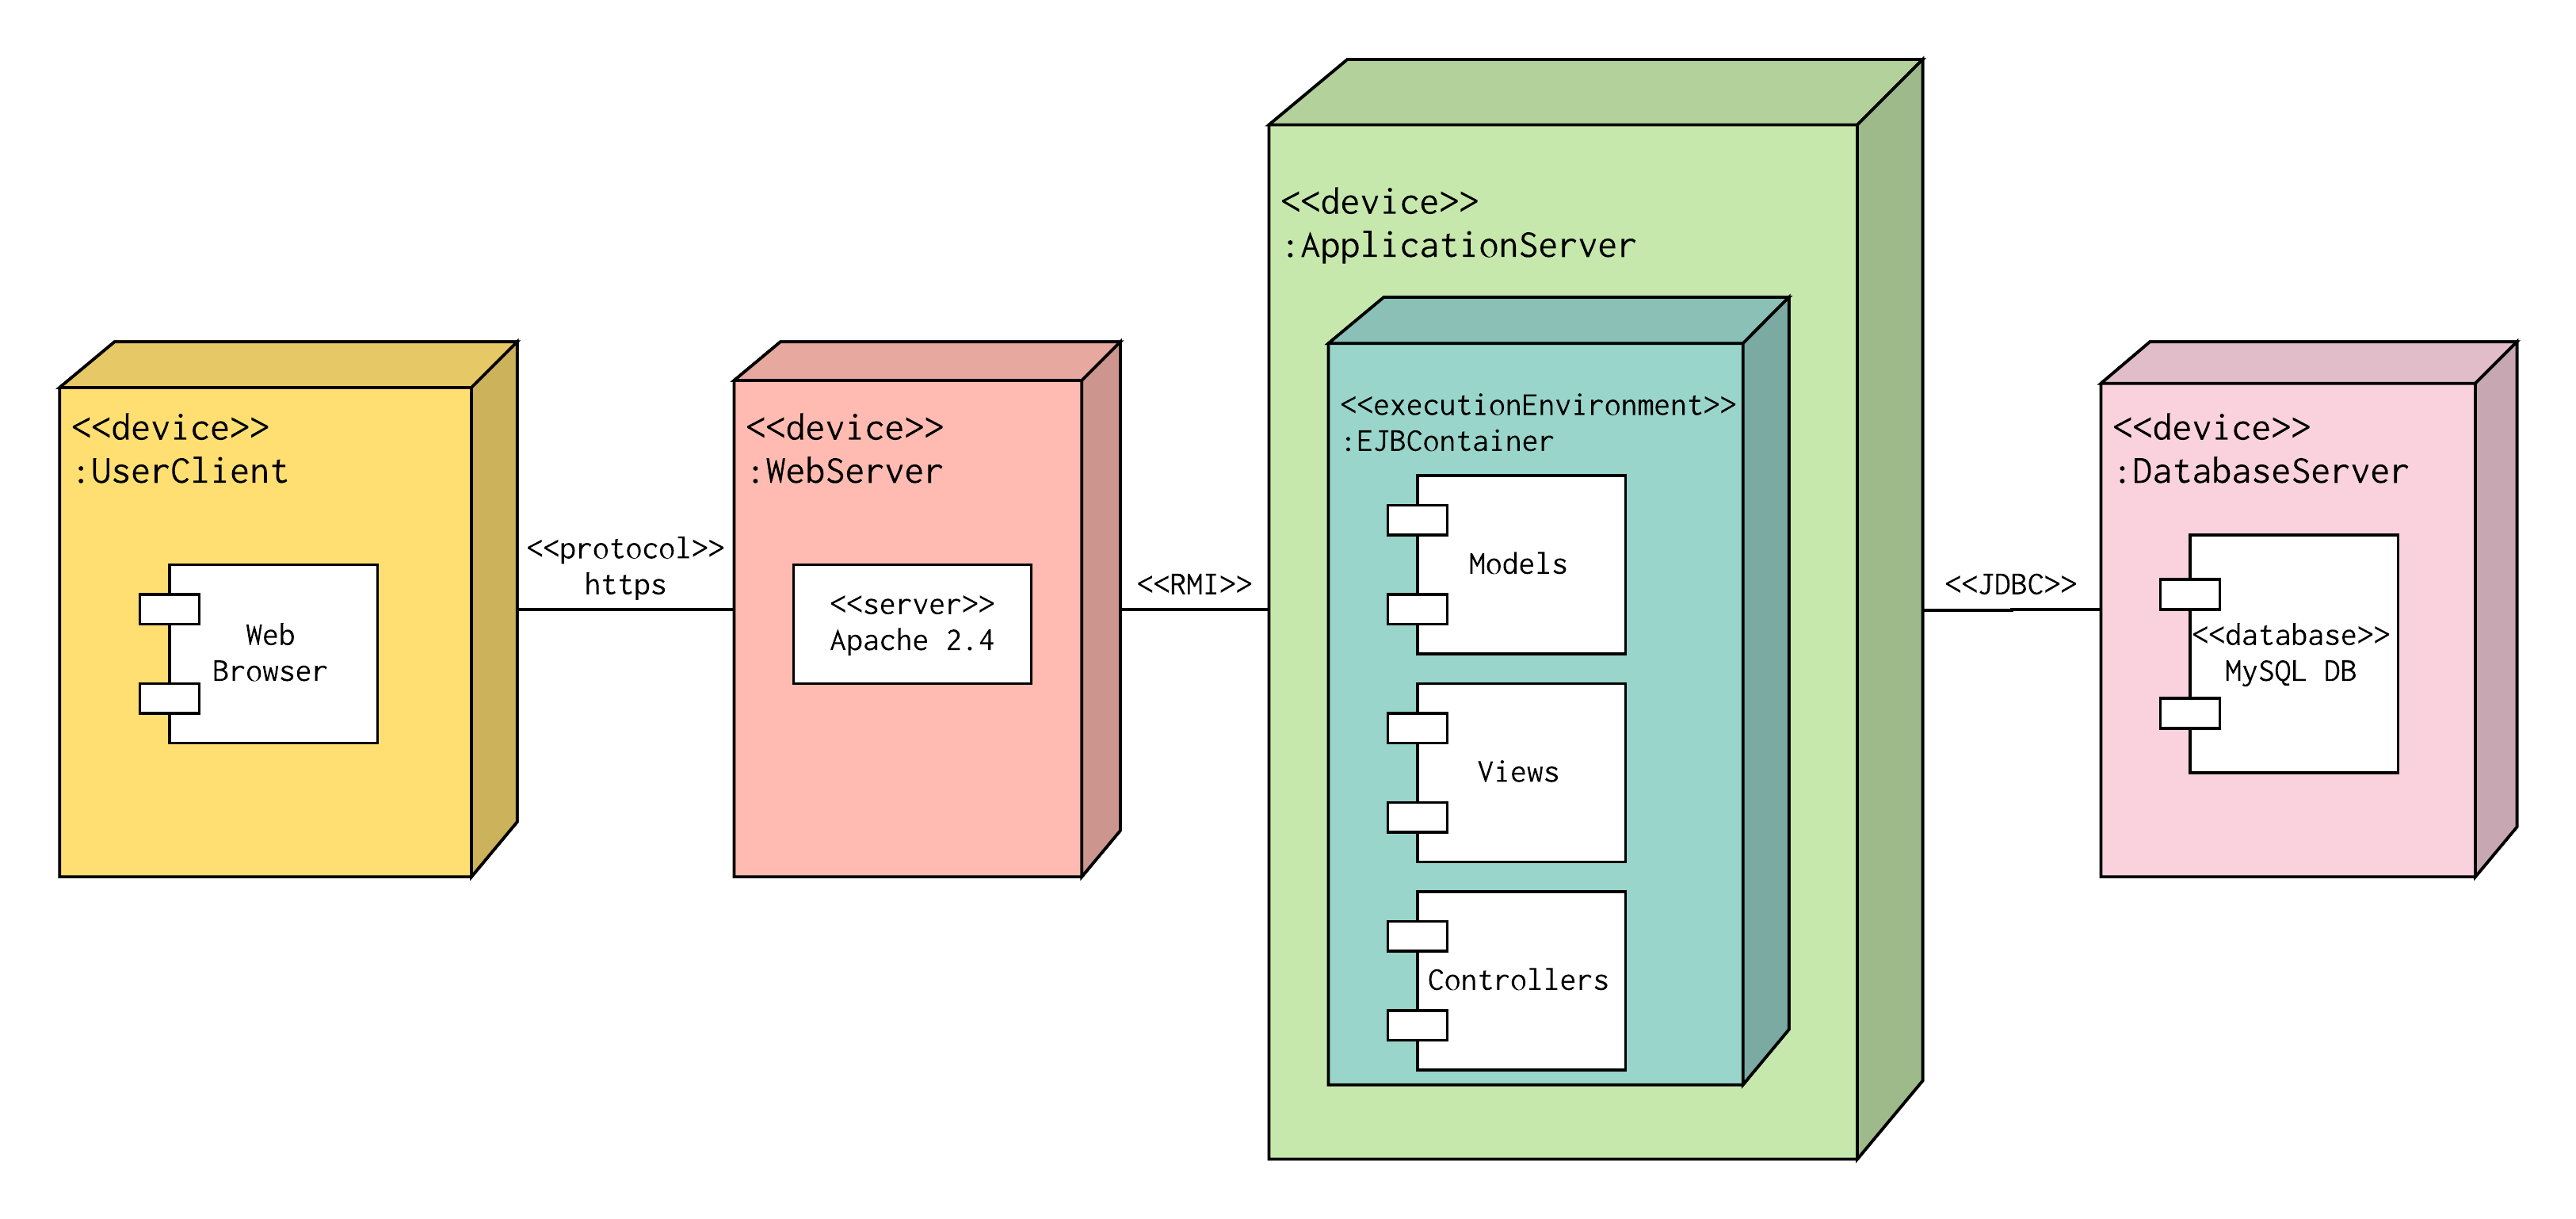
\includegraphics[width=17cm]{img/deployment_diagram.png}
    \caption{Deployment Diagram}
    \label{deployment_diagram}
\end{figure}

\section{Site Map}

The hierarchical structure of the system is depicted in the following site map. It shows the organisation of the site's content and provides a good overview of the pages of the site.

\begin{figure}[H]
    \centering
    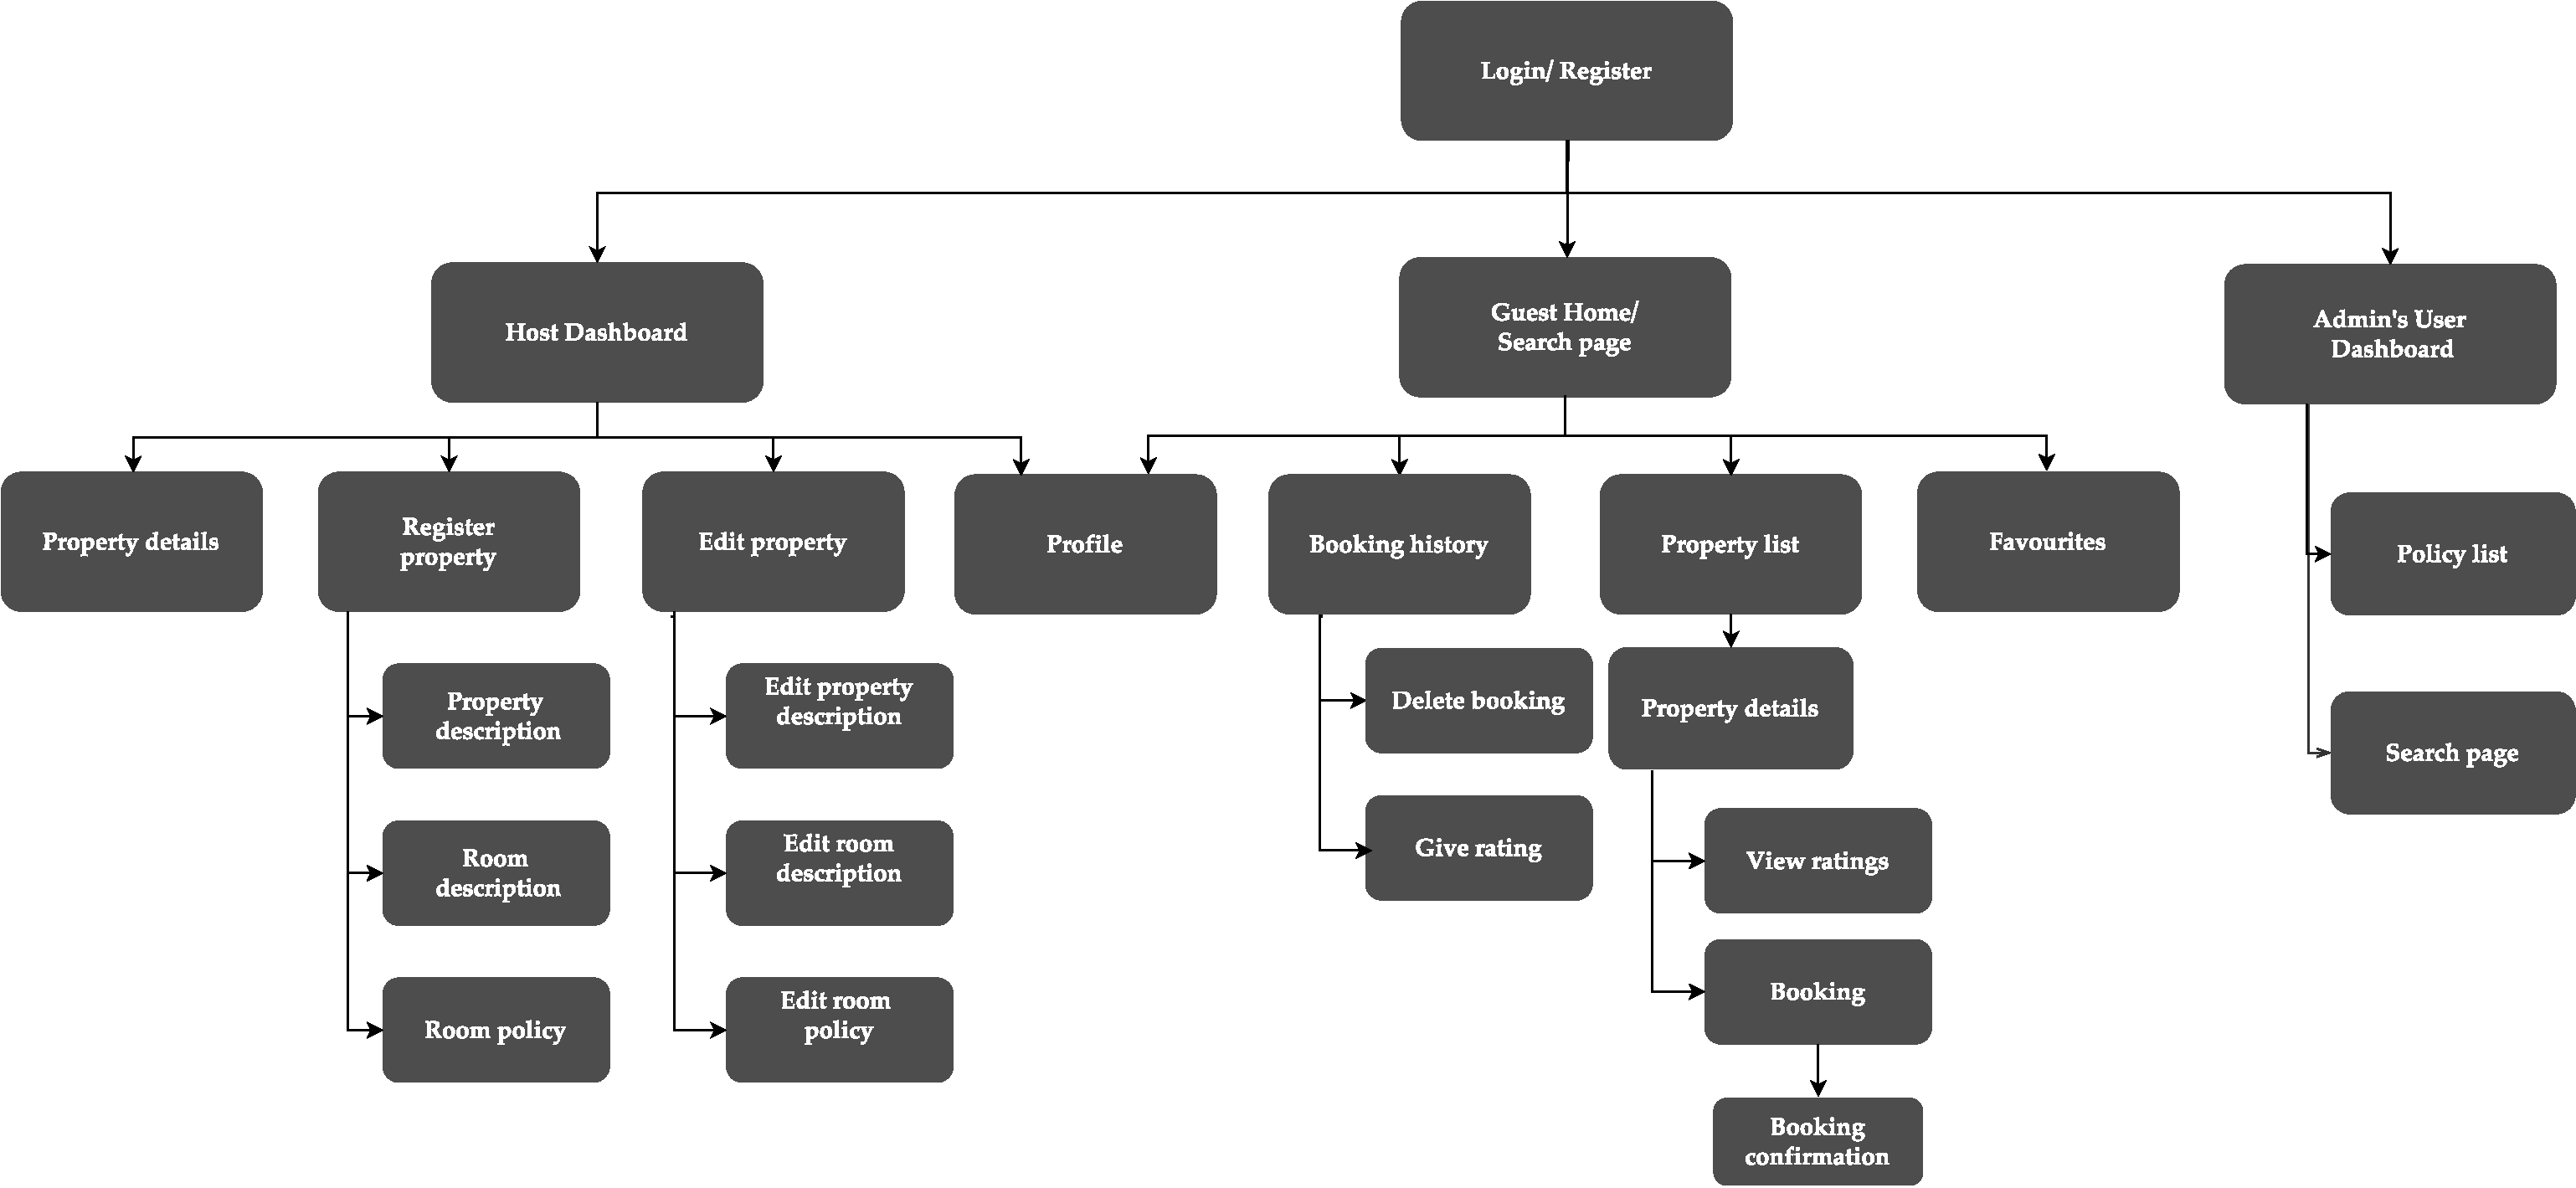
\includegraphics[width=17cm]{img/site_map.pdf}
    \caption{Site Map}
    \label{site_map}
\end{figure}